% LaTeX Template for short student reports.
% Citations should be in bibtex format and go in references.bib
\documentclass[a4paper, 11pt]{article}
\usepackage[top=3cm, bottom=3cm, left = 2cm, right = 2cm]{geometry} 
\geometry{a4paper} 
\usepackage[utf8]{inputenc}
\usepackage{textcomp}
\usepackage{graphicx} 
\usepackage{amsmath,amssymb}  
\usepackage{bm}  
\usepackage[pdftex,bookmarks,colorlinks,breaklinks]{hyperref}  
\hypersetup{linkcolor=black,citecolor=black,filecolor=black,urlcolor=black} % black links, for printed output
\usepackage{memhfixc} 
\usepackage{pdfsync}  
\usepackage{fancyhdr}
\usepackage{fancyvrb}
\usepackage{natbib}
\usepackage{url}
%\pagestyle{fancy}
\usepackage{tabto}
\usepackage[shortlabels]{enumitem}
\usepackage{tikz}
\usepackage{verbatim}
\usepackage{nameref}
\usepackage{caption}
\usepackage{subcaption}
\usepackage{mathtools}
\usepackage{hyperref}
\usepackage{soul}

\title{Concrete Earth: A DirectX Game}
\author{Sam Drysdale}
\date{May 16, 2023}

\begin{document}
\graphicspath{{./Images/}}
\maketitle
\tableofcontents
\begin{flushleft}

\section{Summary}

\textit{Concrete Earth} is a game about nuclear semiotics. Ostensibly, the story is set in a medieval fiefdom, cursed by the occult ciphers long-etched into its landscape. The twist is this is set millenia \textit{after} a nuclear apocalypse - the `curse' is radiation poisoning, the ciphers the dead language of the previous civilisation, warning of nearby waste repositories. Though it is still in development, this prototype demostrates how the DirectX 11 functionality might bring such a concept to life. Indeed, for a game so concerned with language, it is appropriate that many key features are grounded in linguistics; while the terrain itself is generated by marching cubes, \textit{Concrete Earth} uses grammars to create both procedural screen shaders and a procedural narrative.

\vspace{5pt}\noindent
A video demonstration can be found within the ``docs'' directory, and \href{https://www.youtube.com/watch?v=FbqZv7QruQ4&feature=youtu.be}{\ul{online}}. 

\newpage
\section{User Controls}

The user plays as a carriage driver, journeying forwards over an endless map. Periodically, they will be stopped by a `multiple-choice' scene, where an option must be selected before continuing. Such is the core game loop of \textit{Concrete Earth}.

\vspace{5pt}\noindent
The application uses the following key mappings:\footnote{While the framework registers inputs on press, note that options are only selected \textit{on release}.}

\begin{center}
\parbox[t]{0.75\textwidth}{
\vspace{0pt}\noindent 
\textbf{W} \dotfill{} Move north

\vspace{2.5pt}\noindent 
\textbf{A} \dotfill{} Move northwest

\vspace{2.5pt}\noindent 
\textbf{D} \dotfill{} Move northeast

\vspace{2.5pt}\noindent 
\textbf{1} \dotfill{} Select option \#$1$

\vspace{2.5pt}\noindent 
\textbf{2} \dotfill{} Select option \#$2$

\vspace{2.5pt}\noindent 
\textbf{3} \dotfill{} Select option \#$3$

\vspace{2.5pt}\noindent 
\textbf{Esc} \dotfill{} Quit
}\linebreak
\end{center}

Clicking \textbf{LMB} will also select an option. The application runs at a fixed $1920 \times 1080$ resolution.

\section{Features}\label{Features}

The following is a technical discussion of the key features of \textit{Concrete Earth}, with a focus on its advanced procedural generation. Mathematical models and code snippets are kept to a minimum, edited for clarity rather than accuracy to the original application.

%\subsection{Noise} % TECHNIQUE: Perlin/simplex noise...

\subsection{Procedural Terrain}\label{Procedural Terrain} % TECHNIQUE: Marching cubes...

Given the concept, this game's terrain is of course intended to evoke a sense of ``shunned land'' \citep{trth93}. In generating the jutting thorns and blocks so essential to the post-nuclear setting, though, there comes a problem - concavity. Height maps are perfectly adequate for creating rolling hills and valleys, but the fact that each of their $(x,z)$-coordinates can correspond to only one $y$-value would prevent any overhangs in \textit{Concrete Earth}'s barren landscape (see Figure \ref{Concave Terrain}).

%\vspace{5pt}\noindent
\begin{figure}[h]
\centering
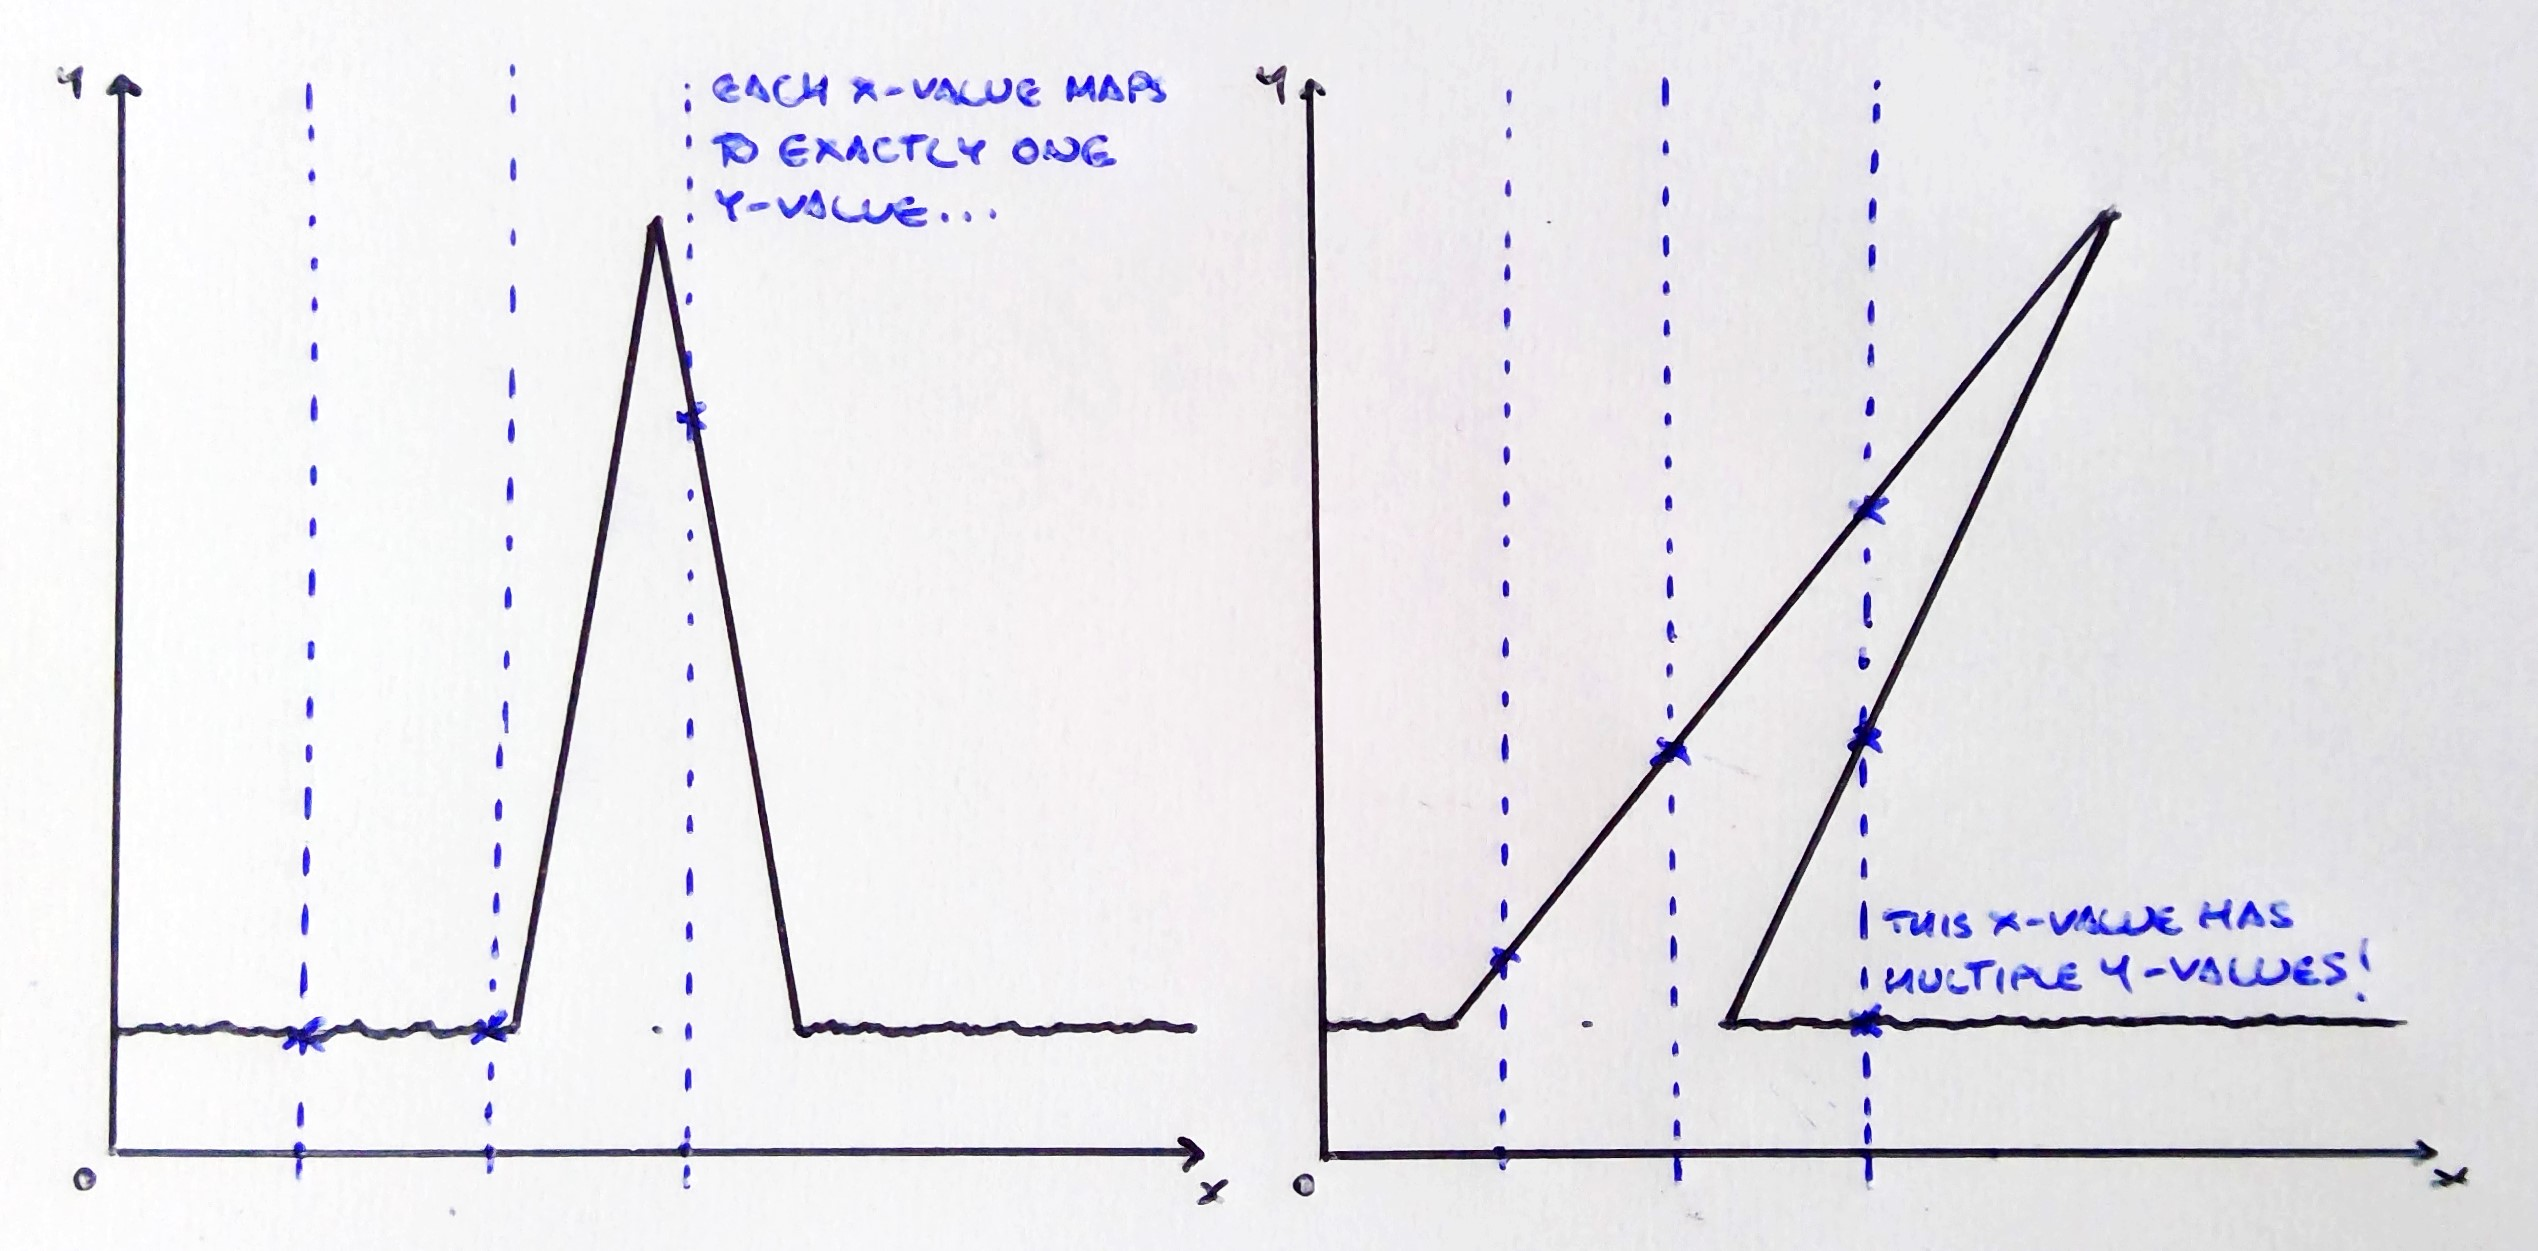
\includegraphics[width=0.66\textwidth]{Concave Terrain}
\caption{Two sketches of `thorny' terrain; the former can be generated by a height map, whereas the latter is too concave.}
\label{Concave Terrain}
\end{figure}

%\newpage\noindent
%\vspace{5pt}\noindent
\begin{figure}[t]
\centering
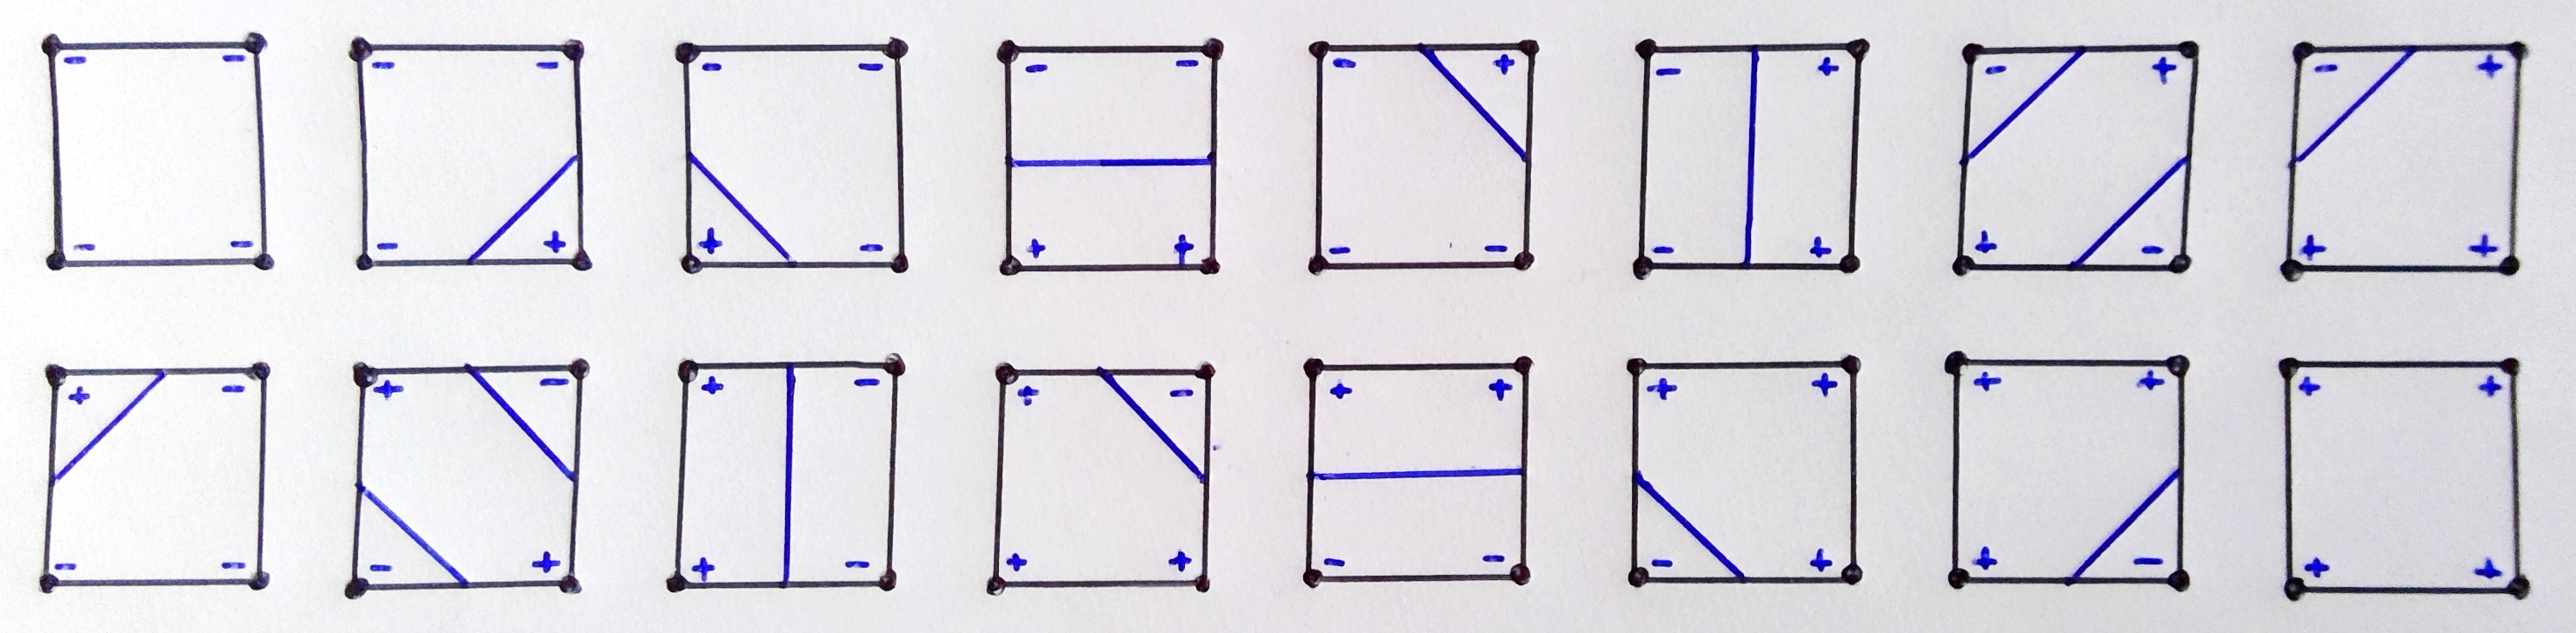
\includegraphics[width=0.9\textwidth]{Marching Square Partitions}
\caption{Linear partitions of a marching square. With $4$ gridpoints, each existing in one of $2$ states (`$+$' for $f_{i,j} \geqslant c$, `$-$' for $f_{i,j} < c$), exactly $2^4 = 16$ partitions are possible.} % NB: $4$, ignoring symmetries!
\label{Marching Square Partitions}
\end{figure}

%\vspace{5pt}\noindent
\begin{figure}[t]
\centering
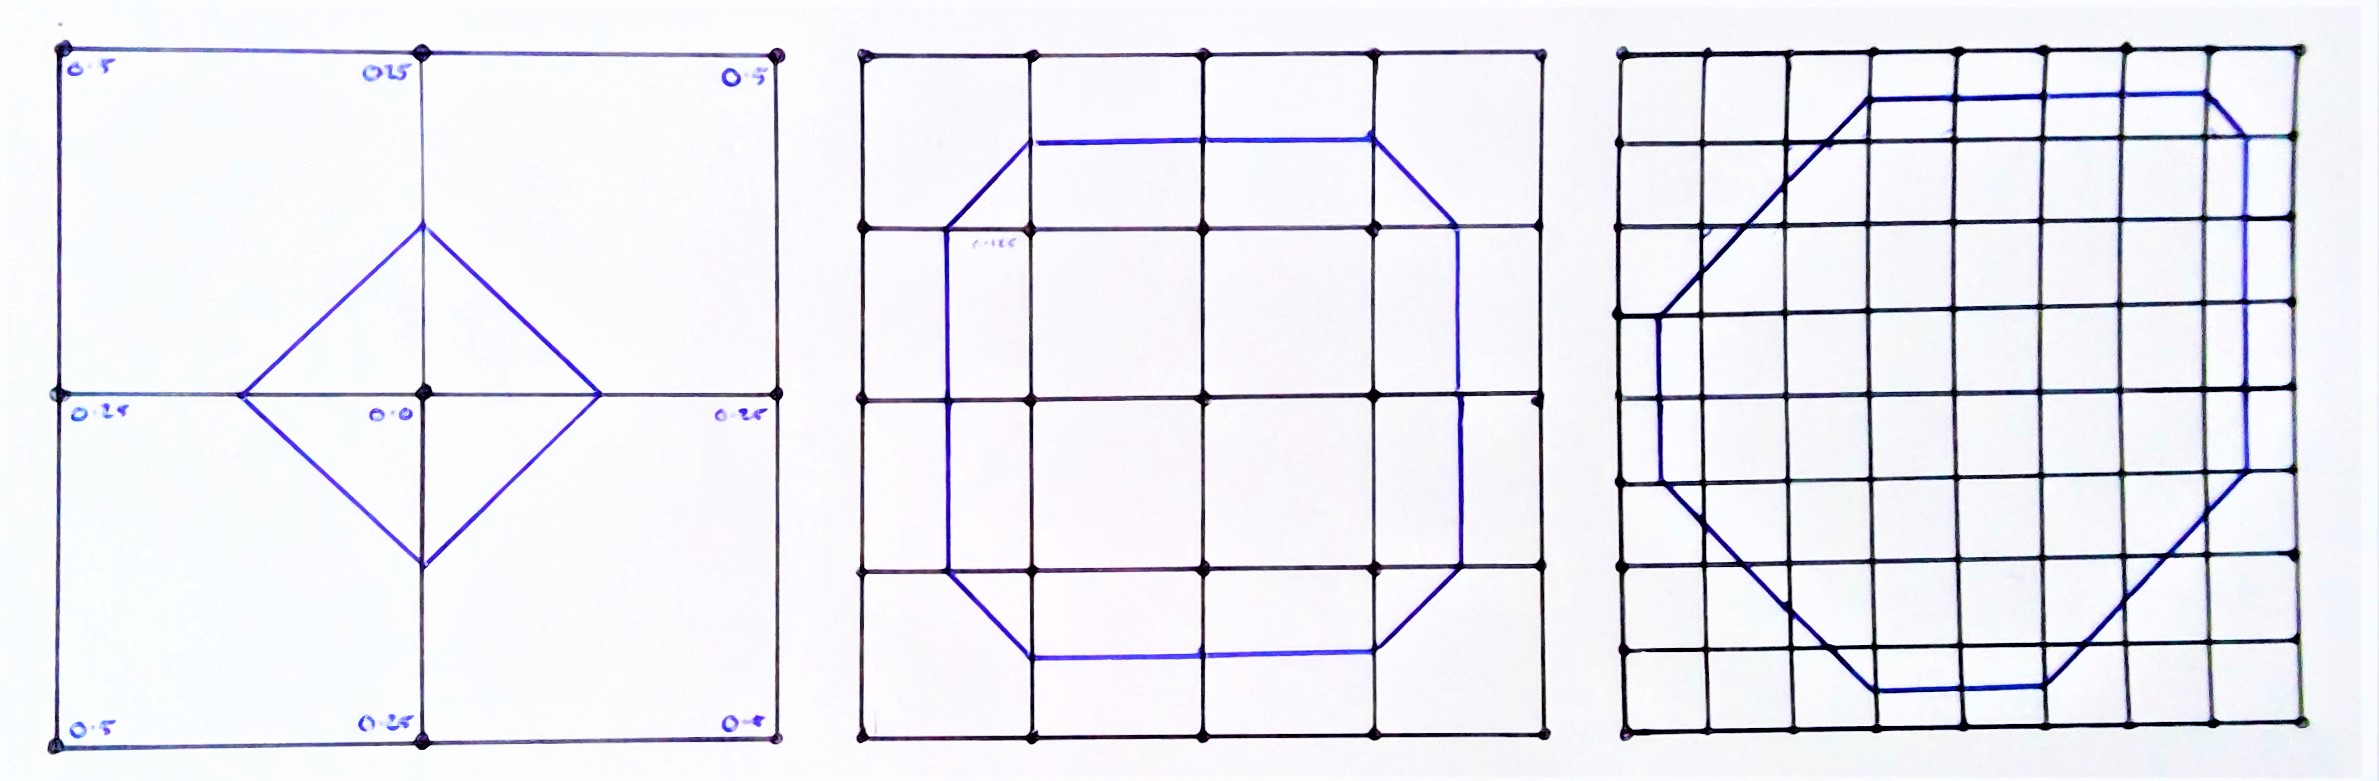
\includegraphics[width=0.9\textwidth]{Marching Squares}
\caption{Bounding curve $f(x,y) = 0.16$, at increasing levels of granularity.}
\label{Marching Squares}
\end{figure}


%\vspace{5pt}\noindent
%\newpage\noindent
Take the two-dimensional analogue of this problem: how does one construct the bounding curve of a (potentially concave, or even disconnected) area? Consider an $n \times n$ square grid, with $n \in \mathbb{N}$,\footnote{This could equally be an $n \times m$ grid; keeping the dimensions the same is just neater.} and let a scalar field $f : [0,1]^2 \rightarrow \mathbb{R}$ assign each gridpoint $(i,j)$ a corresponding value $f_{i,j} = f(i/n,j/n)$. Figure \ref{Marching Square Partitions} shows how to partition a cell so as to enclose the gridpoints with $f_{i,j} < c$ constant. Drawing such a partition into every cell of the grid will therefore approximate the \textit{isoline}\footnote{Informally, a `contour line' of the $2D$ field.} $f(x,y) = c$, with increasing accuracy as $n \rightarrow \infty$.%In each cell of the grid, straight lines can be drawn to  For each square cell, a line can be Consider%Under this construction, it is possible to approximate the \textit{isoclines}\footnote{Informally, the `contour lines' of the field.} $f(x,y) = c$ constant. Suppose%[By partitioning each of the $n \times n$ square cells according to which of its four gridpoints have $f_{i,j} < c$ (see Figure \ref{Marching Square Partitions}), an increasingly accurate curve emerges as $n \rightarrow \infty$.]



\vspace{5pt}\noindent
This is the \textit{marching squares} algorithm, so named for how it uses a \texttt{for} loop to `march through' and fill in each of the $n \times n$ square cells. Figure \ref{Marching Squares}, for example, illustrates how it might apply to 
$$f(x,y) = \min\left(\left(x-0.5\right)^2+\left(y-0.5\right)^2,4\left(\left(x-0.75\right)^2+\left(y-0.75\right)^2\right)\right),$$
a scalar field describing two overlapping circles.


\vspace{5pt}\noindent
%\newpage\noindent
Given adjacent gridpoints $\mathbf{a}$, $\mathbf{b}$ such that $f_{\mathbf{a}} < c < f_{\mathbf{b}}$, Figure \ref{Marching Square Partitions} would have their partitioning line bisect edge $AB$ exactly. However, knowing the partition represents an isoline, this accidentally implies $f\left(0.5\mathbf{a} + 0.5\mathbf{b}\right) \approx c$, which may not be true of the scalar field. Using the standard, first-order approximation that $f$ is linear over short distances 
$$f\left((1-t)\mathbf{a} + t\mathbf{b}\right) \approx c, \,\, \textrm{where} \,\, t = \frac{c-f_{\mathbf{a}}}{f_{\mathbf{b}}-f_{\mathbf{a}}}.$$
Understanding that it is therefore more accurate for the partition to intersect $AB$ at $(1-t)\mathbf{a} + t\mathbf{b}$, such linear interpolation is integrated into the marching squares algorithm (see Figure \ref{Interpolated Marching Squares}).

\begin{figure}[h]
\centering
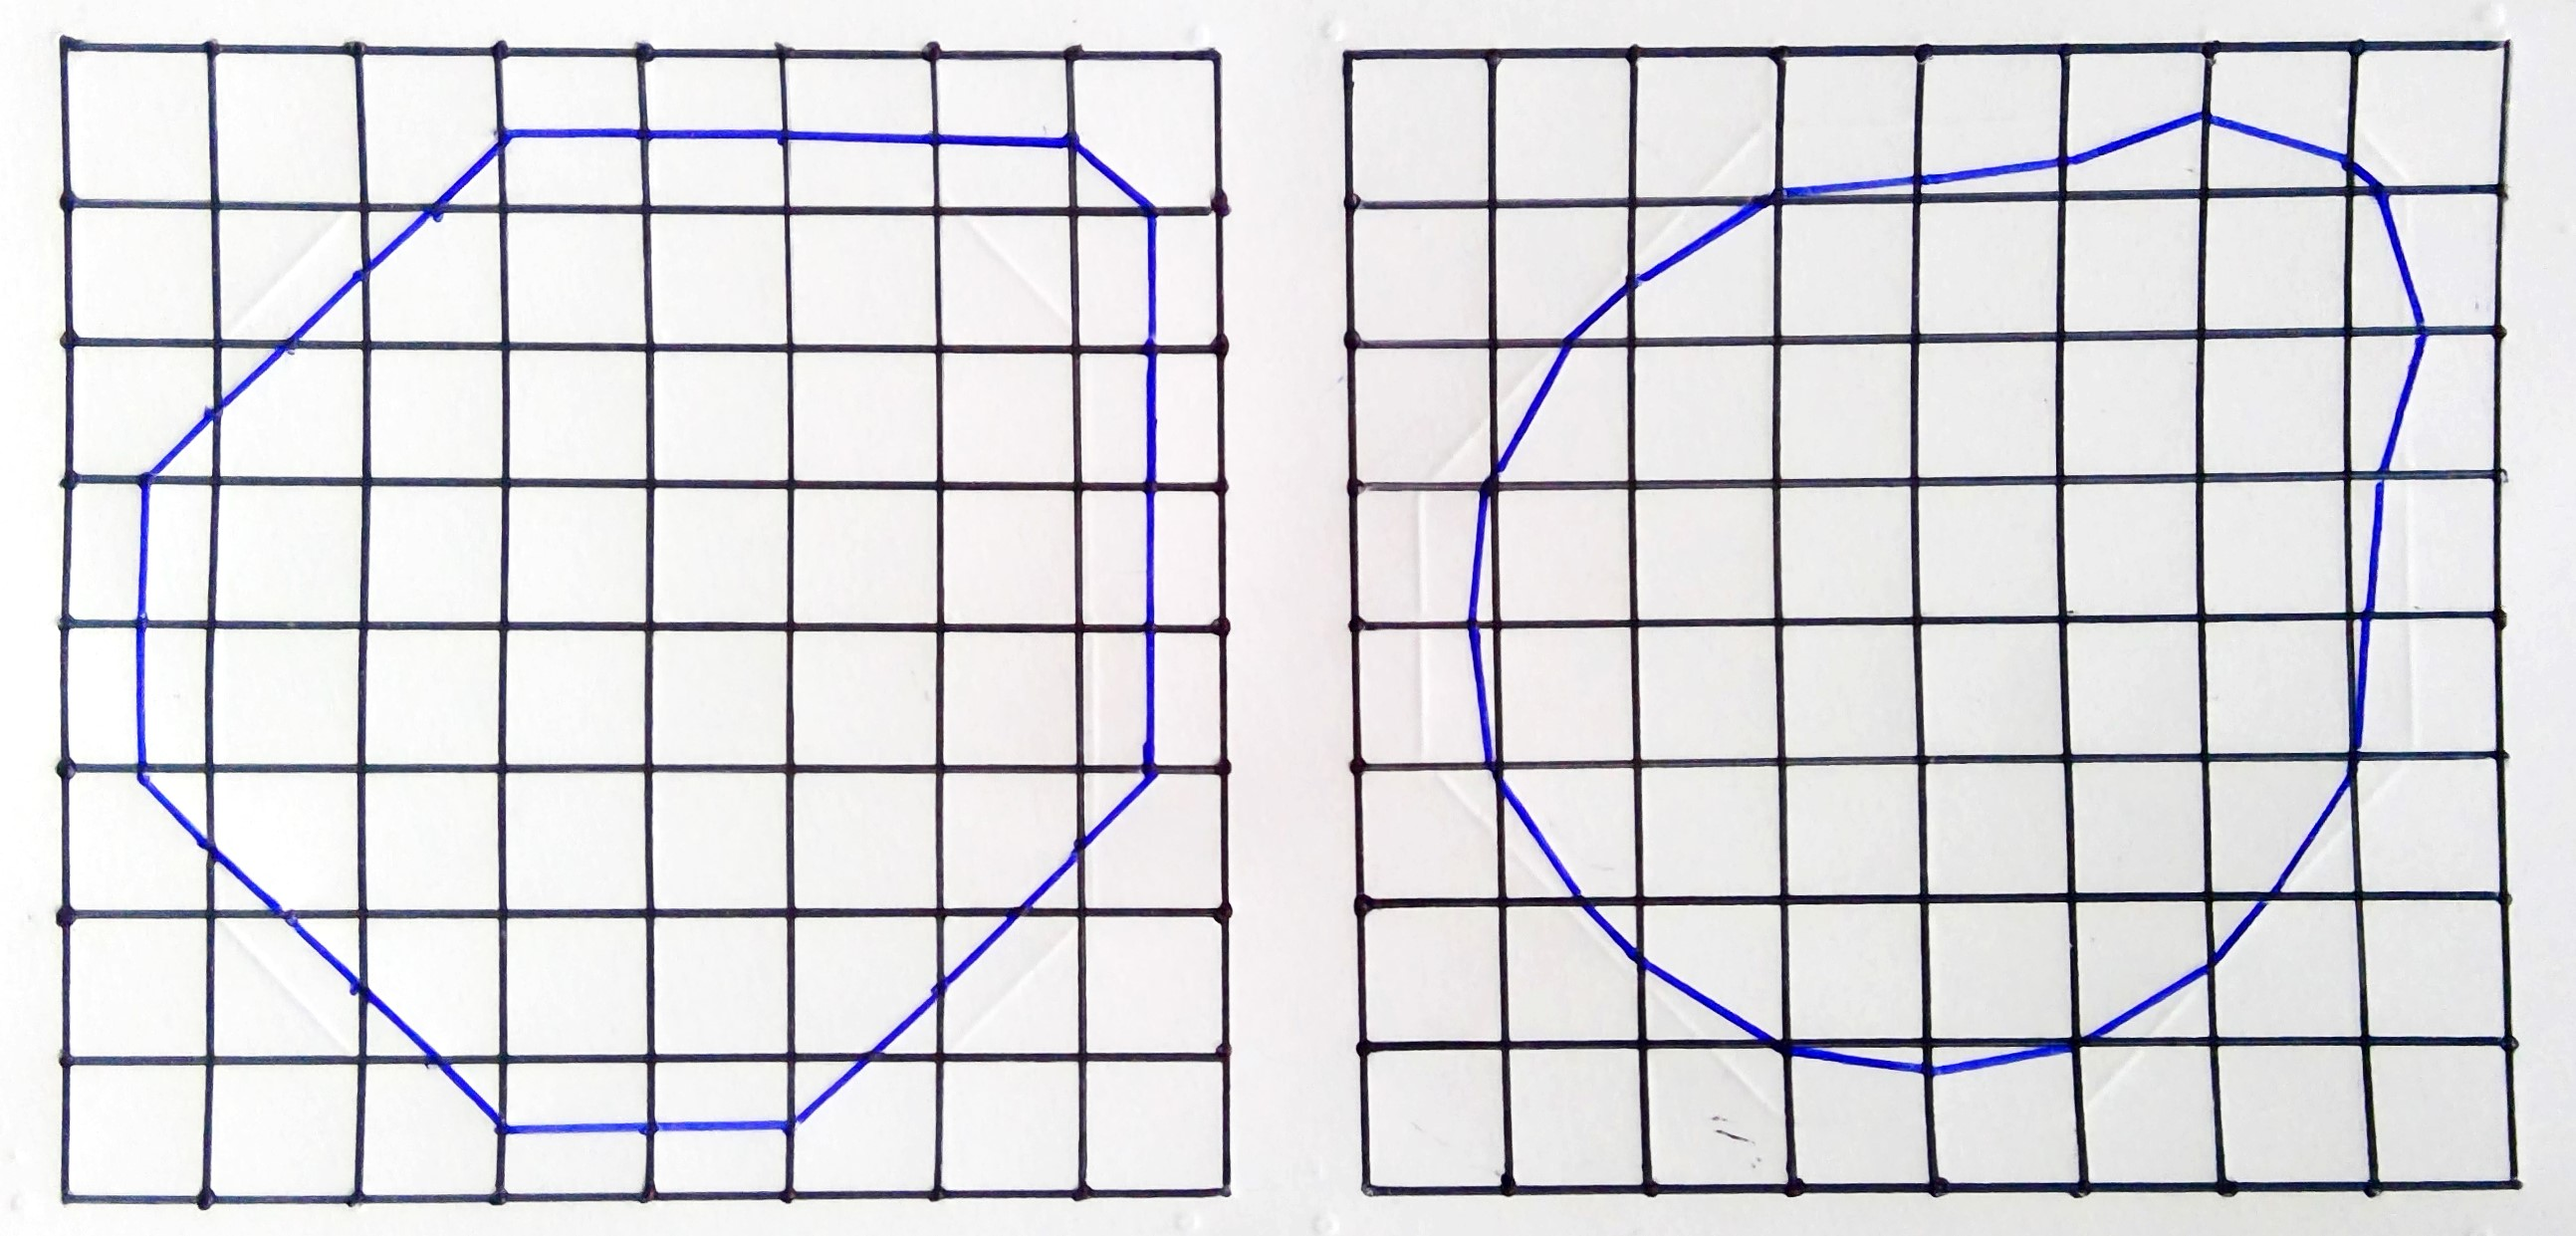
\includegraphics[width=0.66\textwidth]{Interpolated Marching Squares}
\caption{Bounding curve $f(x,y) = 0.16$, before and after linear intepolation.}
\label{Interpolated Marching Squares}
\end{figure}

%\vspace{5pt}\noindent
Returning to the problem at hand, \textit{Concrete Earth} uses \textit{marching cubes} to generate the \textit{isosurfaces} bounding 3D volumes. This requires an $n \times n \times n$ grid, and a new field $f: \left[0,1\right]^3 \rightarrow \mathbb{R}$, the algorithm now filling cubic cells with planar surfaces to partition out the gridpoints $(i,j,k)$ satisfying $f_{i,j,k} < c$ (again using linear interpolation to best approximate  the `true' isosurface). Since 3D fields can be hard to visualise, marching cubes are best understood in relation to marching squares. The intuition established above is readily generalised to higher dimensions; whatever the superficial differences, the guiding principle remains the same.

\vspace{5pt}\noindent
This section will not cover the finer points of the DirectX marching cubes implementation - not how it deconstructs partitioning surfaces into triangles for the vertex/index buffers, nor how it identifies adjacent marching cubes so as to calculate `smooth' vertex normals\footnote{A weighted average is taken over the surface normals of the surrounding triangular faces. If a face has vertices $\mathbf{a}$, $\mathbf{b}$, $\mathbf{c}$, it will be weighted by $1/|(\mathbf{b}-\mathbf{a})\times(\mathbf{c}-\mathbf{a})|$, proportional to the inverse of its area}. The report is only interested in this technique as it relates to \textit{Concrete Earth}'s terrain. Paul \citeauthor{bourkeMarchingCubes}'s \textit{Polygonising a Scalar Field} \citeyearpar{bourkeMarchingCubes} remains the definitive source on the algorithm itself. %, and one that this project's code relies on heavily.

\begin{figure}[h]
\centering
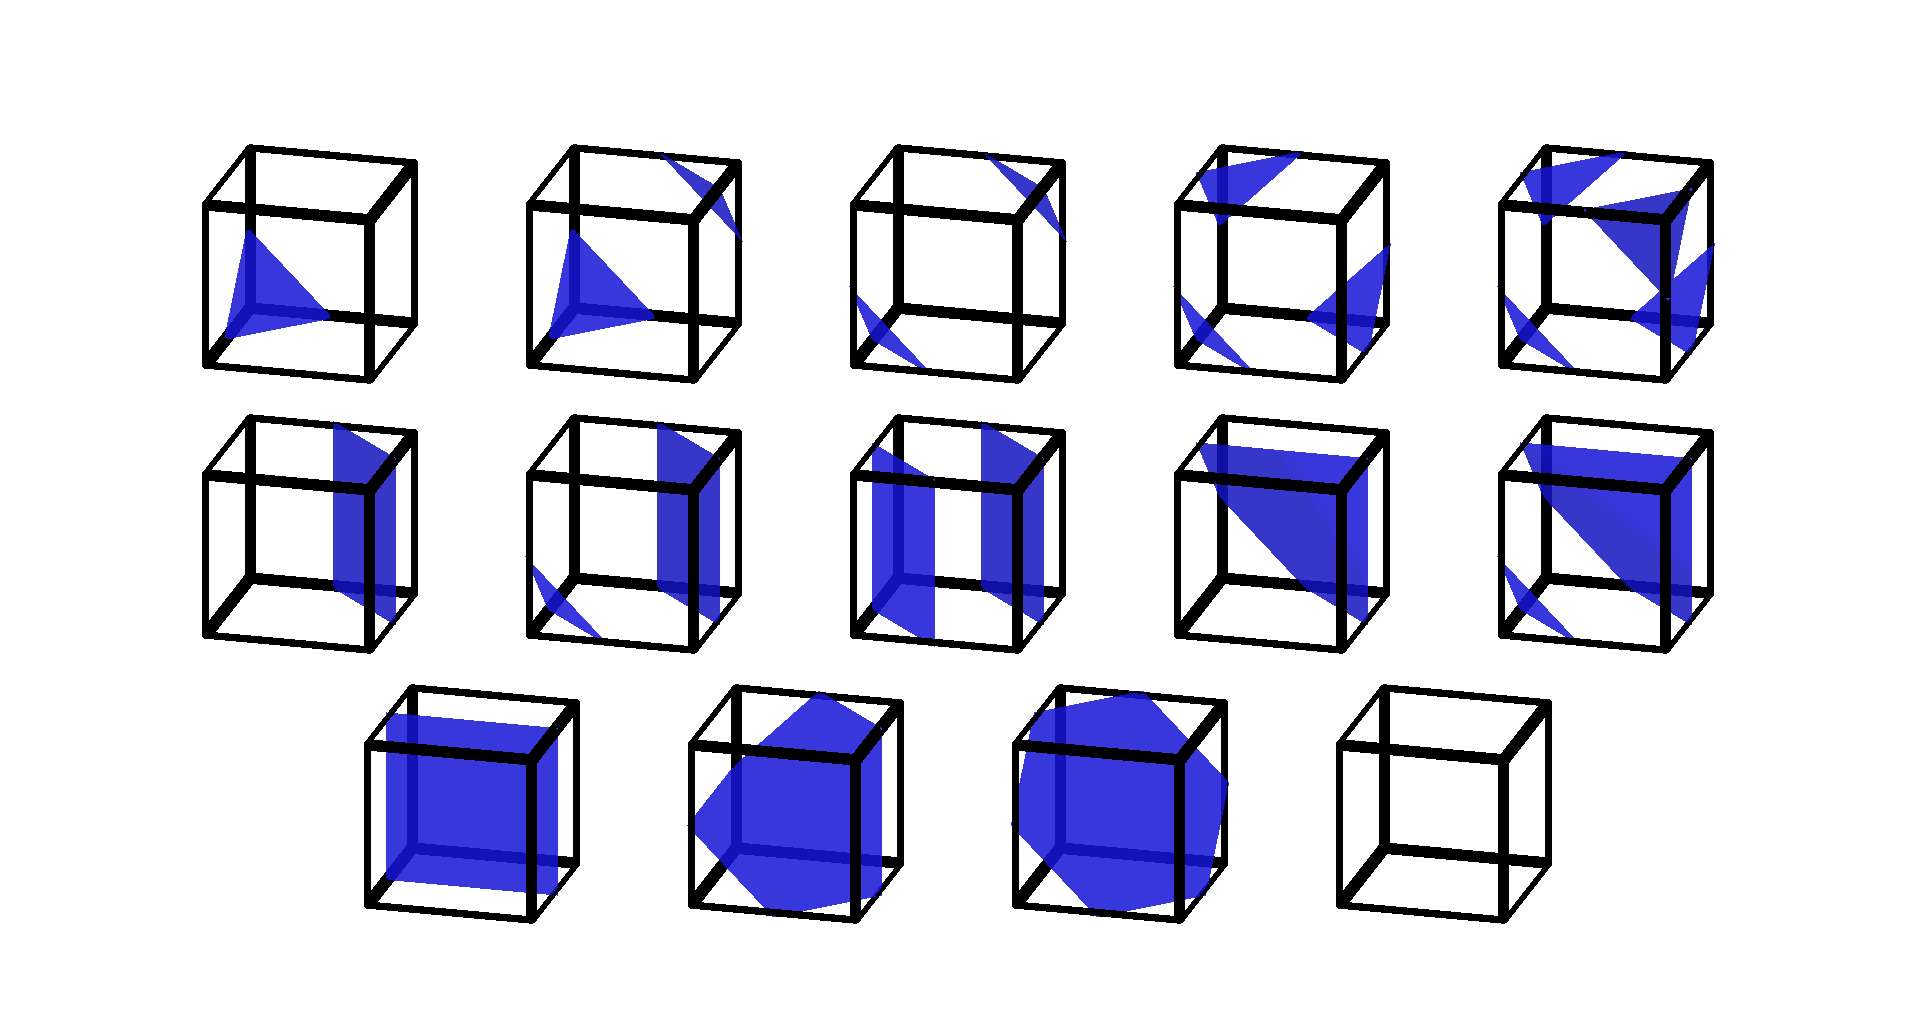
\includegraphics[width=0.75\textwidth]{Marching Cube Partitions}
\caption{Planar partitions of a marching cube, before linear interpolation. There are $14$ fundamental cases, ignoring symmetries; the code itself considers all $2^8 = 256$ possible configurations.}
\label{Marching Cube Partitions}
\end{figure}

\newpage
\subsubsection{Case Study: Hexes}

Having now established a \texttt{MarchingCubes} class, generating a landscape becomes a matter of writing the right scalar field. Indeed, the first step is easyl: for any isovalue $c \in \left(0,1\right)$,
$$\textbf{Height}(\mathbf{x}) = y + 0.1\cdot\textbf{FBM}(\mathbf{x})$$
models a stark, sweeping tundra, its \textit{fractal brownian motion} component scaled to add roughness whilst avoiding `floating islands'. The application treats the underlying simplex noise as a black box.

\vspace{5pt}\noindent
Taking a stylised approach, \textit{Concrete Earth} presents its terrain not as a contiguous mass, but as a board of isometric, hexagonal tiles. To that extent, it relies equally on the second field
$$\textbf{Hex}(\mathbf{x}) = \frac{\sqrt{(2x-1)^2+(2z-1)^2}\cos\left((\theta\bmod\pi/3)-\pi/6\right)}{\cos\left(\pi/6\right)}, \,\, \textrm{where} \,\, \theta = \textrm{arctan2}\left(2z-1, 2x-1\right).$$
For all the trigonometry, this just describes a vertical hexagonal prism centred at $x = 0.5$, $z = 0.5$, much the same as $\sqrt{(2x-1)^2+(2z-1)^2}$ describes a cylinder (see Figure \ref{Hex Field}).
$$\textbf{Terrain}_c(\mathbf{x}) = \max\left(\textbf{Height}(\mathbf{x}), \, c\cdot\textbf{Hex}(\mathbf{x})\right)$$
then takes a maximum to enclose only those gridpoints that fall below the isovalue in \textit{both} fields, imposing hexagonal bounds on the existing terrain (the scale factor of $c$ normalising the width of this hex for all isovalues). 

%\vspace{5pt}\noindent
%[Bounding hexagonal prism... As much as flat faces are antithetical to marching cubes (if they run parallel to the grid, then... can't interpolate? notice that interpolation doesn't account for the degenerate case where two adjacent gridpoints are equal)...] 

\vspace{5pt}\noindent
\begin{figure}[t]
\centering
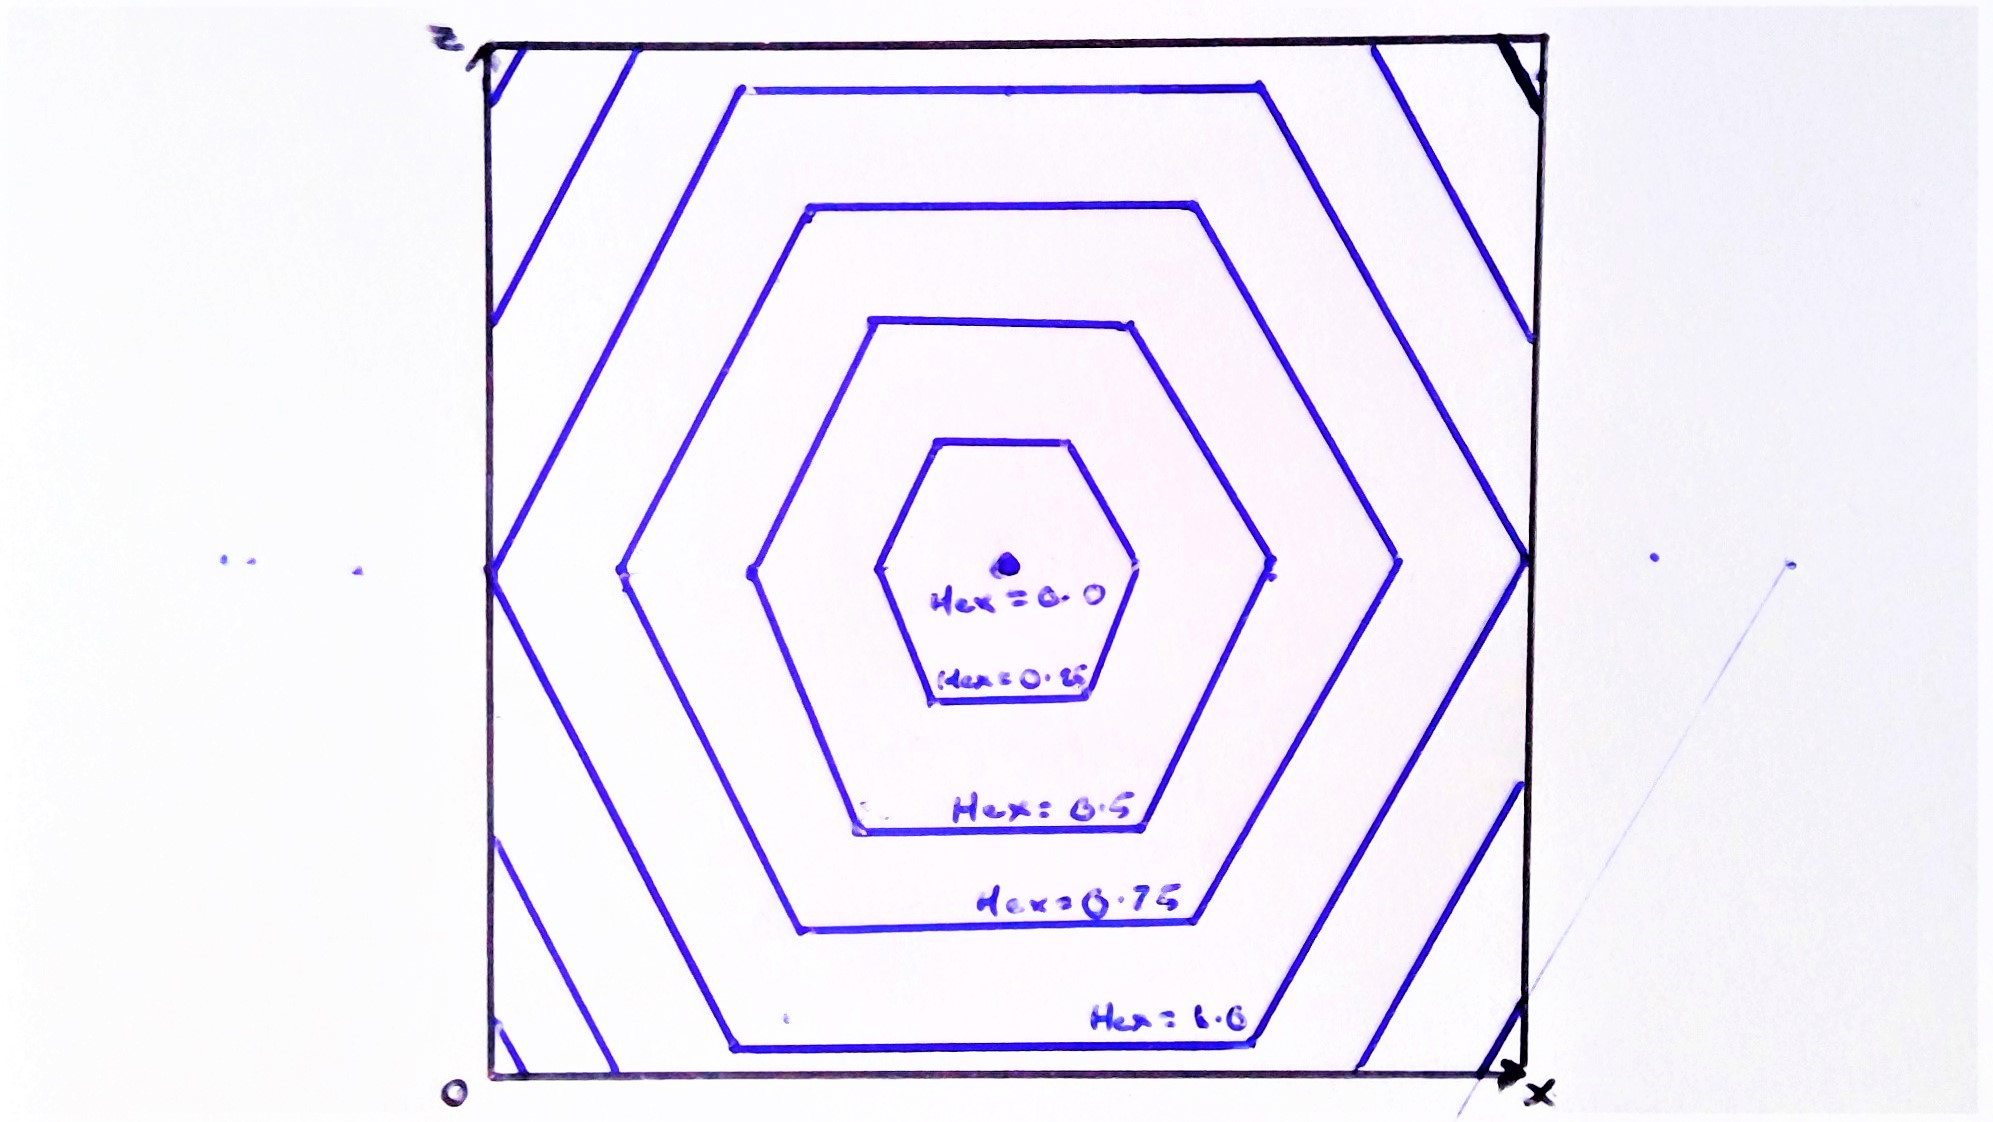
\includegraphics[width=0.66\textwidth]{Hex Field}
\caption{Isolines of $\textbf{Hex}(x,y_0,z)$, a horizontal slice of the hexagonal field.}
\label{Hex Field}
\end{figure}

\subsubsection{Case Study: Landmarks}

Physical markers are similarly integrated. To generate one of the afore-mentioned thorns with apex $\mathbf{a}$, base centred on $\mathbf{b}$, and half angle $\phi$, for instance, the framework defines field

$$\textbf{Thorn}_{\mathbf{a},\mathbf{b},\phi}(\mathbf{x}) = \frac{1}{\phi}\arccos\left(\frac{\left(\mathbf{x}-\mathbf{a}\right)\cdot\left(\mathbf{b}-\mathbf{a}\right)}{\left|\mathbf{x}-\mathbf{a}\right|\cdot\left|\mathbf{b}-\mathbf{a}\right|}\right).$$
Using a minimum, isosurfaces of
$$\textbf{Landmarked Terrain}_{c;\,\mathbf{a},\mathbf{b},\phi}(\mathbf{x}) = \min\left(\textbf{Terrain}_c(\mathbf{x}), \, c\cdot\textbf{Thorn}_{\mathbf{a},\mathbf{b},\phi}(\mathbf{x})\right),$$
contain all gridpoints below the isovalue of \textit{either} field, adding volume just as a maximum subtracts.\footnote{These operations do not commute! Taking the maximum first allows thorns that `stick out' from the bounding hex - this is a conscious, if purely aesthetic, decision on the part of the game.} %Though only a few such fiel have been modelled, 


\vspace{5pt}\noindent
The \texttt{Hex} class handling high-level field generation adds a stochastic element, randomising $\mathbf{a}$, $\mathbf{b}$, $\phi$. Moreover, any number of thorns can be added; taking the minimum over more than two fields just expands the isosurface further. Perhaps the only surprising choice made in procedurally generating these landmarks is keeping their surfaces completely smooth. Rather than simulating weathering and erosion, the conceit of \textit{Concrete Earth} is that these strange, idealised geometries feel distinctly unnatural. The physical markers of shunned land are man-made designs that \textit{should} tap into a sense of the uncanny, in the hopes of communicating to future civilisations that `THIS IS NOT A PLACE OF HONOUR'.  %Only the . Rather than add noise, the game [Explain how we add randomness to thorns]. That said, [smooth, geometric structure].

\vspace{5pt}\noindent
\begin{figure}[h]
\centering
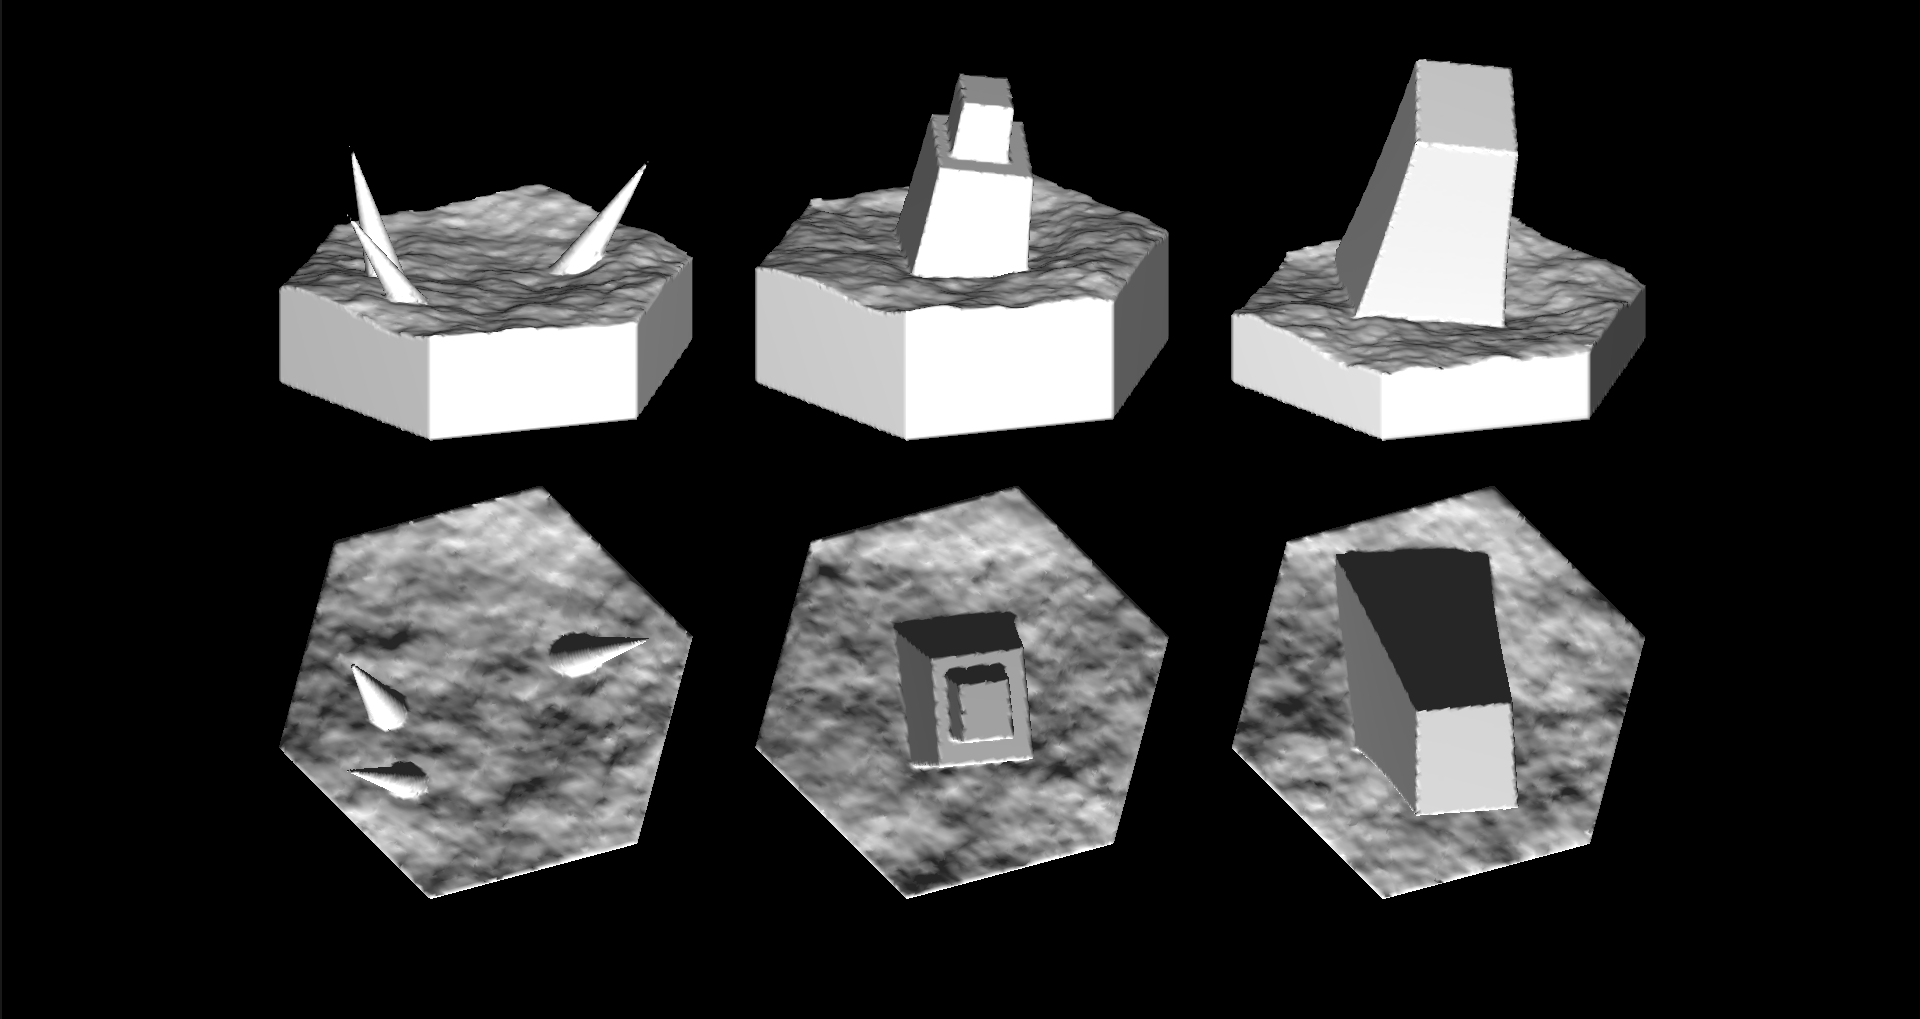
\includegraphics[width=0.66\textwidth]{Landmarks}
\caption{\textit{Concrete Earth}'s landmarks.  Three designs have been prototype so far, with more to be added now the terrain pipeline is feature-complete.}
\label{Landmarks}
\end{figure}

\subsection{Procedural Screen Shaders}\label{Procedural Screen Shaders} % TECHNIQUE: L-systems...

The post-processing in \textit{Concrete Earth} is, in many respects, trivial. \texttt{vignette\_ps.hlsl}, for instance, demands only two renders-to-texture on every frame: the board itself, and an alpha map of blood vessels sprouting from the edges of the screen. As striking as the final effect is, the shader is surprisingly straightforward in blending the textures into a single, pulsing eye strain overlay; far more worthy of further discussion is how the blood vessels themselves are generated.

\newpage\noindent
%\vspace{5pt}\noindent
In formal languages, a grammar is a tuple $G = (N,\Sigma,P,\omega_0)$. This contains two disjoint sets of symbols: nonterminals $A, B, \dots \in N$, and terminals $a, b, \dots \in \Sigma$. The production rules in $P$ map nonterminals to strings $\alpha, \beta, \dots \in (N\cup\Sigma)^*$; applied recursively to the axiom $\omega_0 \in (N\cup\Sigma)^*$, these rules can produce increasingly complex \textit{sentences} of terminals and/or nonterminals.\footnote{In mathematical literature, $
\omega_0 \in N$ \citep*{hopcroftFormalLanguages}, but this project takes an informal approach.}

\vspace{5pt}\noindent
The Chomsky hierarchy \citep{chomskyHierarchy} % NB: Is this *strictly* true?
classifies grammars by their production rules:
\begin{enumerate}[label=,itemsep=0em]
\item \textit{Type-3}. \textit{Regular grammars} map $A \mapsto a$ or $A \mapsto aB$.
\item \textit{Type-2}. \textit{Context-free grammars} map $A \mapsto \alpha$.
\item \textit{Type-1}. \textit{Context-sensitive grammars} $\alpha A\beta \mapsto \alpha\gamma\beta$.
\item \textit{Type-0}. \textit{Unrestricted grammars} map $\alpha \mapsto \beta$, where $\alpha$ is non-empty.
\end{enumerate}
Note that all Type-3 grammars are also Type-2, all Type-2 grammars also Type-1, and so on.

\vspace{5pt}\noindent
Suppose, for example, that $N = \{F, G\}$, $\Sigma = \{+, -\}$, $P = \{F \mapsto F+G, G \mapsto F-G\}$, $\omega_0 = F$.
Letting $\omega_n$ denote the sentences generated by applying the production rules $n$ times, it follows that
$$\begin{matrix*}[l]
\omega_1 &= &F+G, \\
\omega_2 &= &F+G+F-G, \\
\omega_3 &= &F+G+F-G+F+G-F-G, \\
\omega_4 &= &F+G+F-G+F+G-F-G+F+G+F-G-F+G-F-G, \;\; \cdots.
\end{matrix*}$$

\vspace{5pt}\noindent
While these definitions are rather abstract, \citet{lindenmayerLSystems} provides a remarkable application. Treating each symbol as an instruction like `go forward' or `turn right', \textit{L-systems} visualise sentences using turtle graphics; when the sentences have been generated recursively by a grammar, the line drawings will inherit their self-similar structure. Consider the above example - reading non-terminals $F$, $G$ as `draw a line while moving 1 unit forwards,' and terminals $\pm$ as `turn by $\pm\, \pi/2$ on the spot,' produces dragon curve fractals (see Figure \ref{Dragon Curves}).

\vspace{5pt}\noindent
\begin{figure}[h]
\centering
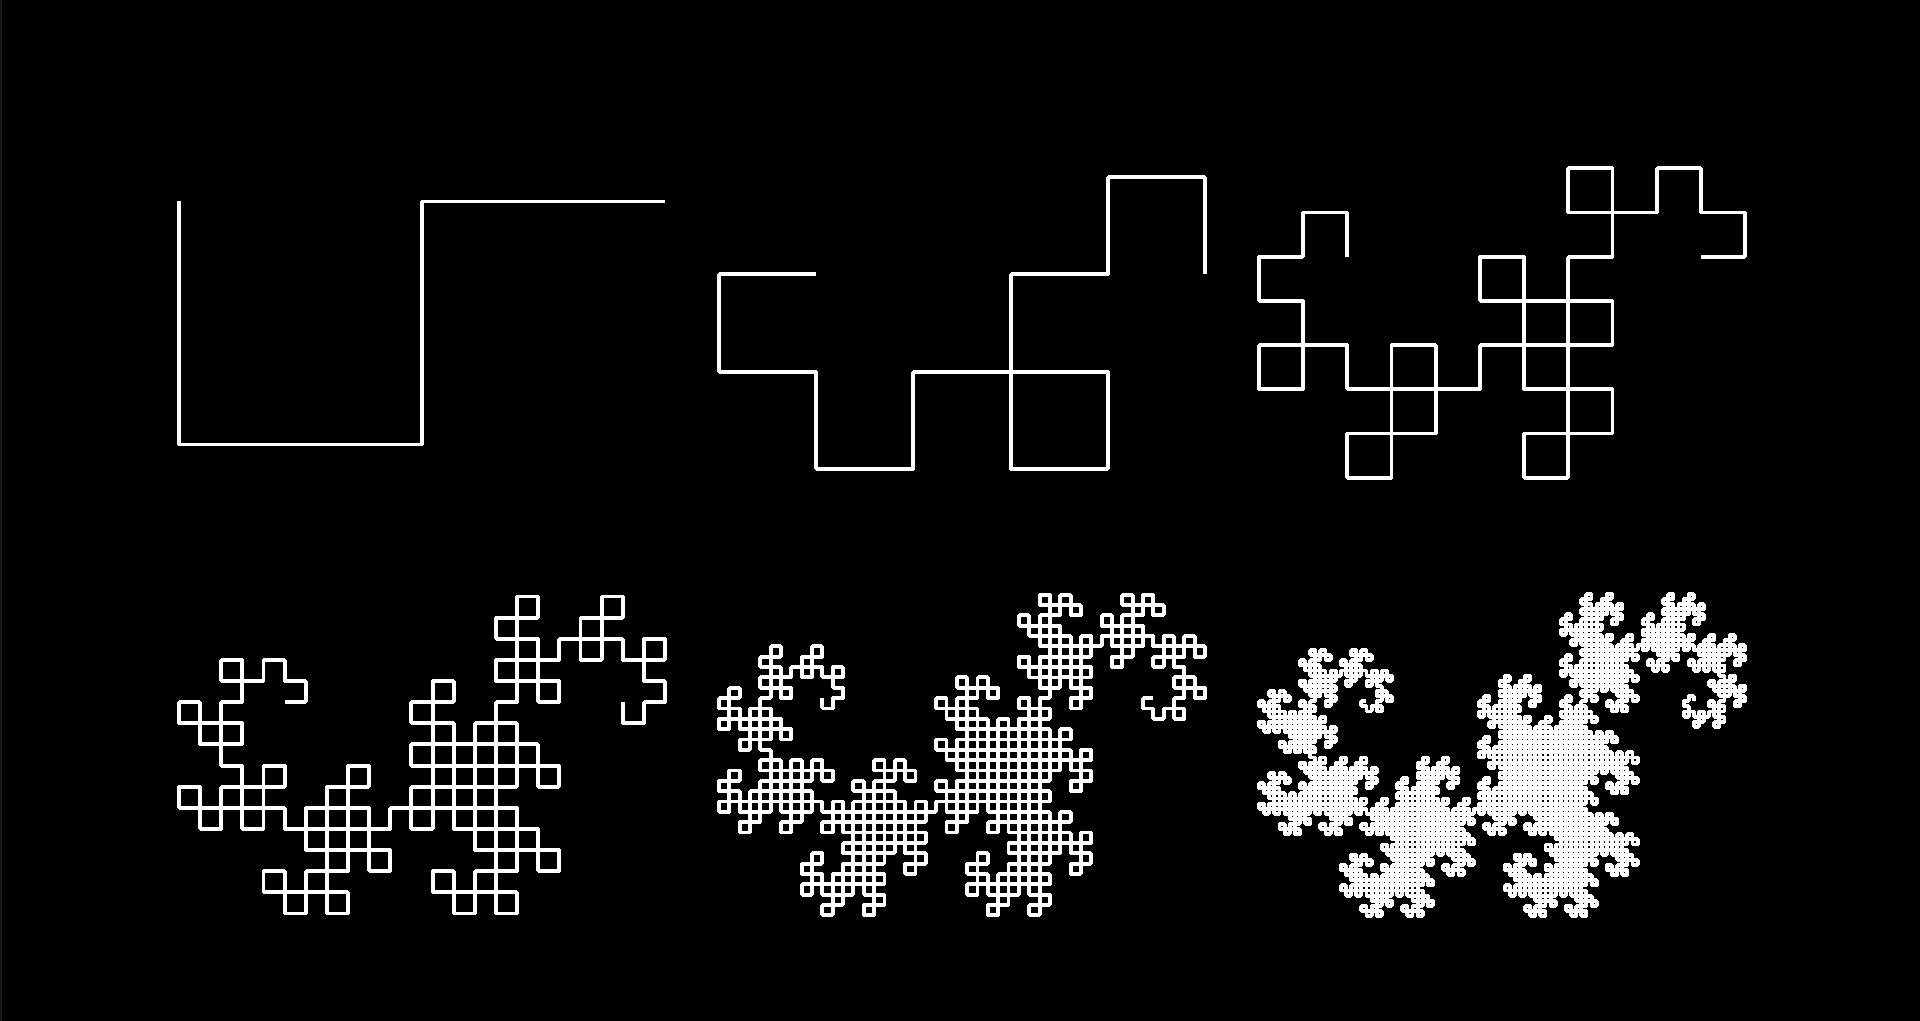
\includegraphics[width=0.66\textwidth]{Dragon Curves}
\caption{Dragon curves, generated by strings $\omega_2, \omega_4, \cdots, \omega_{12}$.}
\label{Dragon Curves}
\end{figure}

\vspace{5pt}\noindent
While L-systems are most common in the modelling of 3D plants and other branching structures \citep{prusinkiewiczAlgorithmicBeauty}, \textit{Concrete Earth} only uses them to generate 2D alpha maps. Moreover, it restricts its attention to L-systems paired with context-free grammars.

\subsubsection{Case Study: Blood Vessels}

Generalising the above, \textit{parametric L-systems} act not on symbols $A$ but \textit{modules} $\mathbf{A}(x_1,\cdots,x_n)$. By treating non-terminals as structures containing parameters $x_1$, $\cdots$, $x_n$, production rules can then be written to act on said parameters.

\vspace{5pt}\noindent
This project's own \texttt{LSystem} class tracks three main values: the length $l$, width $w$, and orientation $\theta$ with which to draw each line segment. The benefit is, if nothing else, organisational. Even in the basic L-system for dragon curves, terminals $\pm$ are made redundant by the altogether more readable set of production rules
$$\begin{matrix*}[l]
\mathbf{F}(l,w,\theta) &\mapsto &\mathbf{F}(l,w,\theta)\mathbf{G}(l,w,\theta+\pi/2) \\
\mathbf{G}(l,w,\theta) &\mapsto &\mathbf{F}(l,w,\theta)\mathbf{G}(l,w,\theta-\pi/2).
\end{matrix*}$$

\vspace{5pt}\noindent
\citet{zamirArterialBranchingLSystems}, meanwhile, uses this parametric formulation to visualise bifurcations of blood vessels. Suppose a branch with length $l$, width $w$ bifurcates into two branches $M$ and $m$, such that $l_M \geq l_m$. Defining the \textit{asymmetry ratio} $\alpha = l_m/l_M$, it follows that
$$l_M = \frac{l}{\left(1+\alpha^3\right)^{1/3}}, \;\; l_m = \frac{\alpha\cdot l}{\left(1+\alpha^3\right)^{1/3}}, \;\; w_M = \frac{w}{\left(1+\alpha^3\right)^{1/3}}, \;\; w_m = \frac{\alpha\cdot w}{\left(1+\alpha^3\right)^{1/3}}.$$
Furthermore, the branches diverge from their parent at angles
$$\theta_M = \arccos\left(\frac{\left(1+\alpha^3\right)^{4/3}+1-\alpha^4}{2\left(1+\alpha^3\right)^{2/3}}\right), \;\; \theta_m = \arccos\left(\frac{\left(1+\alpha^3\right)^{4/3}+\alpha^4-1}{2\alpha^2\left(1+\alpha^3\right)^{2/3}}\right).$$
This application is therefore capable of reproducing \citeauthor{zamirArterialBranchingLSystems}'s results (see Figure \ref{Zamir's Model}), using an L-system with the single production rule $\mathbf{C}(l,w,\theta) \mapsto \mathbf{X}(l,w,\theta)[\mathbf{C}(l_M,w_M,\theta+\theta_M)]\mathbf{C}(l_m,w_m,\theta-\theta_m)$.

\vspace{5pt}\noindent
\begin{figure}[h]
\centering
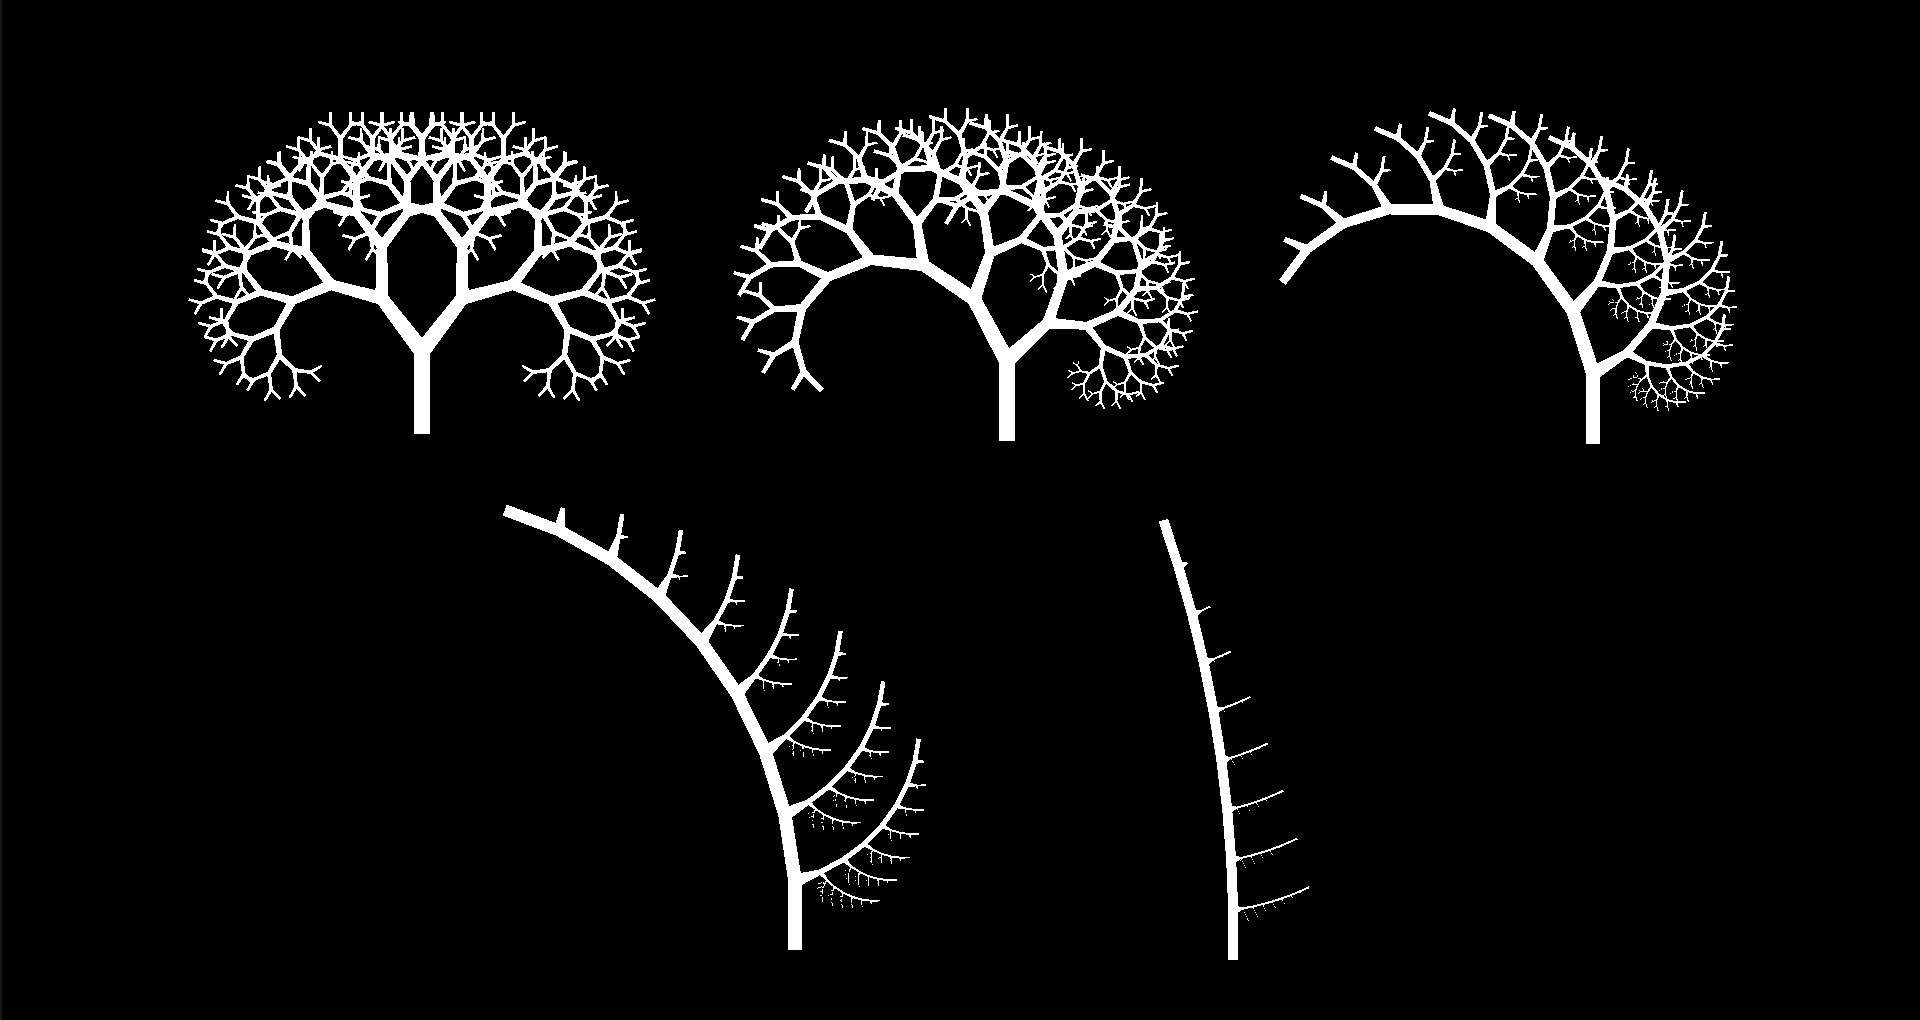
\includegraphics[width=0.66\textwidth]{Zamir's Model}
\caption{\citeauthor{zamirArterialBranchingLSystems}'s model of arterial branching, generated with asymmetry ratios $\alpha = 1.0, 0.8, \cdots, 0.2$. This is an explicit copy of \citeauthor{zamirArterialBranchingLSystems} (\citeyear{zamirArterialBranchingLSystems}, Figure 8), recreated within the DirectX framework.}
\label{Zamir's Model}
\end{figure}

%\vspace{5pt}\noindent
%$$\begin{matrix*}[l]
%\mathbf{C} &\mapsto &\mathbf{X}[+\mathbf{C}]-\mathbf{C} \\
%\mathbf{X} &\mapsto &\mathbf{X}\mathbf{X}
%\end{matrix*}$$

%\vspace{5pt}\noindent
%$$\begin{matrix*}[l]
%\mathbf{C}, \\
%\mathbf{X}[+\mathbf{C}]-\mathbf{C}, \\
%\mathbf{X}\mathbf{X}[+\mathbf{X}[+\mathbf{C}]-\mathbf{C}]-\mathbf{X}[+\mathbf{C}]-\mathbf{C}, \\
%\mathbf{X}\mathbf{X}\mathbf{X}\mathbf{X}[+\mathbf{X}\mathbf{X}[+\mathbf{X}[+\mathbf{C}]-\mathbf{C}]-\mathbf{X}[+\mathbf{C}]-\mathbf{C}]-\mathbf{X}\mathbf{X}[+\mathbf{X}[+\mathbf{C}]-\mathbf{C}]-\mathbf{X}[+\mathbf{C}]-\mathbf{C}, \;\; \cdots
%\end{matrix*}$$

%\vspace{5pt}\noindent
%$$\begin{matrix*}[l]
%\mathbf{C}(l,w,\theta) &\xmapsto[0.4]{} &\mathbf{X}(l,w,\theta)[\mathbf{C}(l_M,w_M,\theta+\theta_M)]\mathbf{C}(l_m,w_m,\theta-\theta_m) \\
%\mathbf{C}(l,w,\theta) &\xmapsto[0.4]{} &\mathbf{X}(l,w,\theta)[\mathbf{C}(l_m,w_m,\theta+\theta_m)]\mathbf{C}(l_M,w_M,\theta-\theta_M) \\
%\mathbf{C}(l,w,\theta) &\xmapsto[0.2]{} &\mathbf{X}(l,w,\theta)\mathbf{C}(l,w,\theta) \\
%\end{matrix*}$$

%\newpage\noindent
\vspace{5pt}\noindent
\citet{liuSimulationBloodVessels} expand on this research with a further stochastic component - they assign \textit{multiple} production rules to a single non-terminal, choosing which to apply using a weighted probability distribution. \textit{Concrete Earth} incorporates such randomness into its own rules for blood vessels:
$$\begin{matrix*}[l]
\mathbf{C}(l,w,\theta) &\xmapsto[0.45]{} &\mathbf{X}(l,w,\theta)[\mathbf{L}(l_M,w_M,\theta+\theta_M)]\mathbf{R}(l_m,w_m,\theta-\theta_m) \\
\mathbf{C}(l,w,\theta) &\xmapsto[0.45]{} &\mathbf{X}(l,w,\theta)[\mathbf{L}(l_m,w_m,\theta+\theta_m)]\mathbf{R}(l_M,w_M,\theta-\theta_M) \\
\mathbf{C}(l,w,\theta) &\xmapsto[0.10]{} &\mathbf{X}(l,w,\theta)\mathbf{C}(l,w,\theta) \\
%& & \\
\mathbf{L}(l,w,\theta) &\xmapsto[1.00]{} &\mathbf{X}(l,w,\theta)\mathbf{C}(l_M,w_M,\theta-\theta_M) \\
%& & \\
\mathbf{R}(l,w,\theta) &\xmapsto[1.00]{} &\mathbf{X}(l,w,\theta)\mathbf{C}(l_M,w_M,\theta+\theta_M)
\end{matrix*}$$
These describe a capillary with a 45\% chance of bifurcating with branch $M$ tacking clockwise, a 45\% chance of bifurcating with $M$ tacking anticlockwise, and a 10\% chance of extending forwards without any branching. The deterministic production rules on $\mathbf{L}$, $\mathbf{R}$ provide course correction, ensuring the models can be pointed towards the centre of the screen without veering off in either direction. Further informal tweaks can be found in the \texttt{LBloodVessel} class itself. 



\vspace{5pt}\noindent
Finally, assigning each \texttt{line} segment a (strictly positive) \texttt{depth} value and taking the \texttt{maxDepth} across all such segments, a normalised \texttt{intensity} factor scales the model as follows: 
\begin{center} % NB: CHECK THIS CODE LINES UP!
\begin{BVerbatim}
for (int i = 0; i < line.size(); i++)
{
    float growth = 1.0f-(1.0f-intensity)*maxDepth/line[i].depth;
    line[i].length *= std::max(0.0f,std::min(growth, 1.0f));
}
\end{BVerbatim}
\end{center}
As \texttt{intensity} increases from \texttt{0.0f} to \texttt{1.0f}, the blood vessels grow, the `deepest' branches emerging first.\footnote{On a more technical level, \textit{Concrete Earth} treats a branch's \texttt{depth} as a function of the \texttt{length}s of its child branches. Though it came about from a typo in the code, the definition stuck - by delaying growth around bifurcation points, it achieve a nice `sprouting' effect!} 
Rendering these to texture results in a visceral, procedurally-animated post-process effect, more responsive than passing in a static alpha map. 

%\vspace{5pt}\noindent
\begin{figure}[h]
\centering
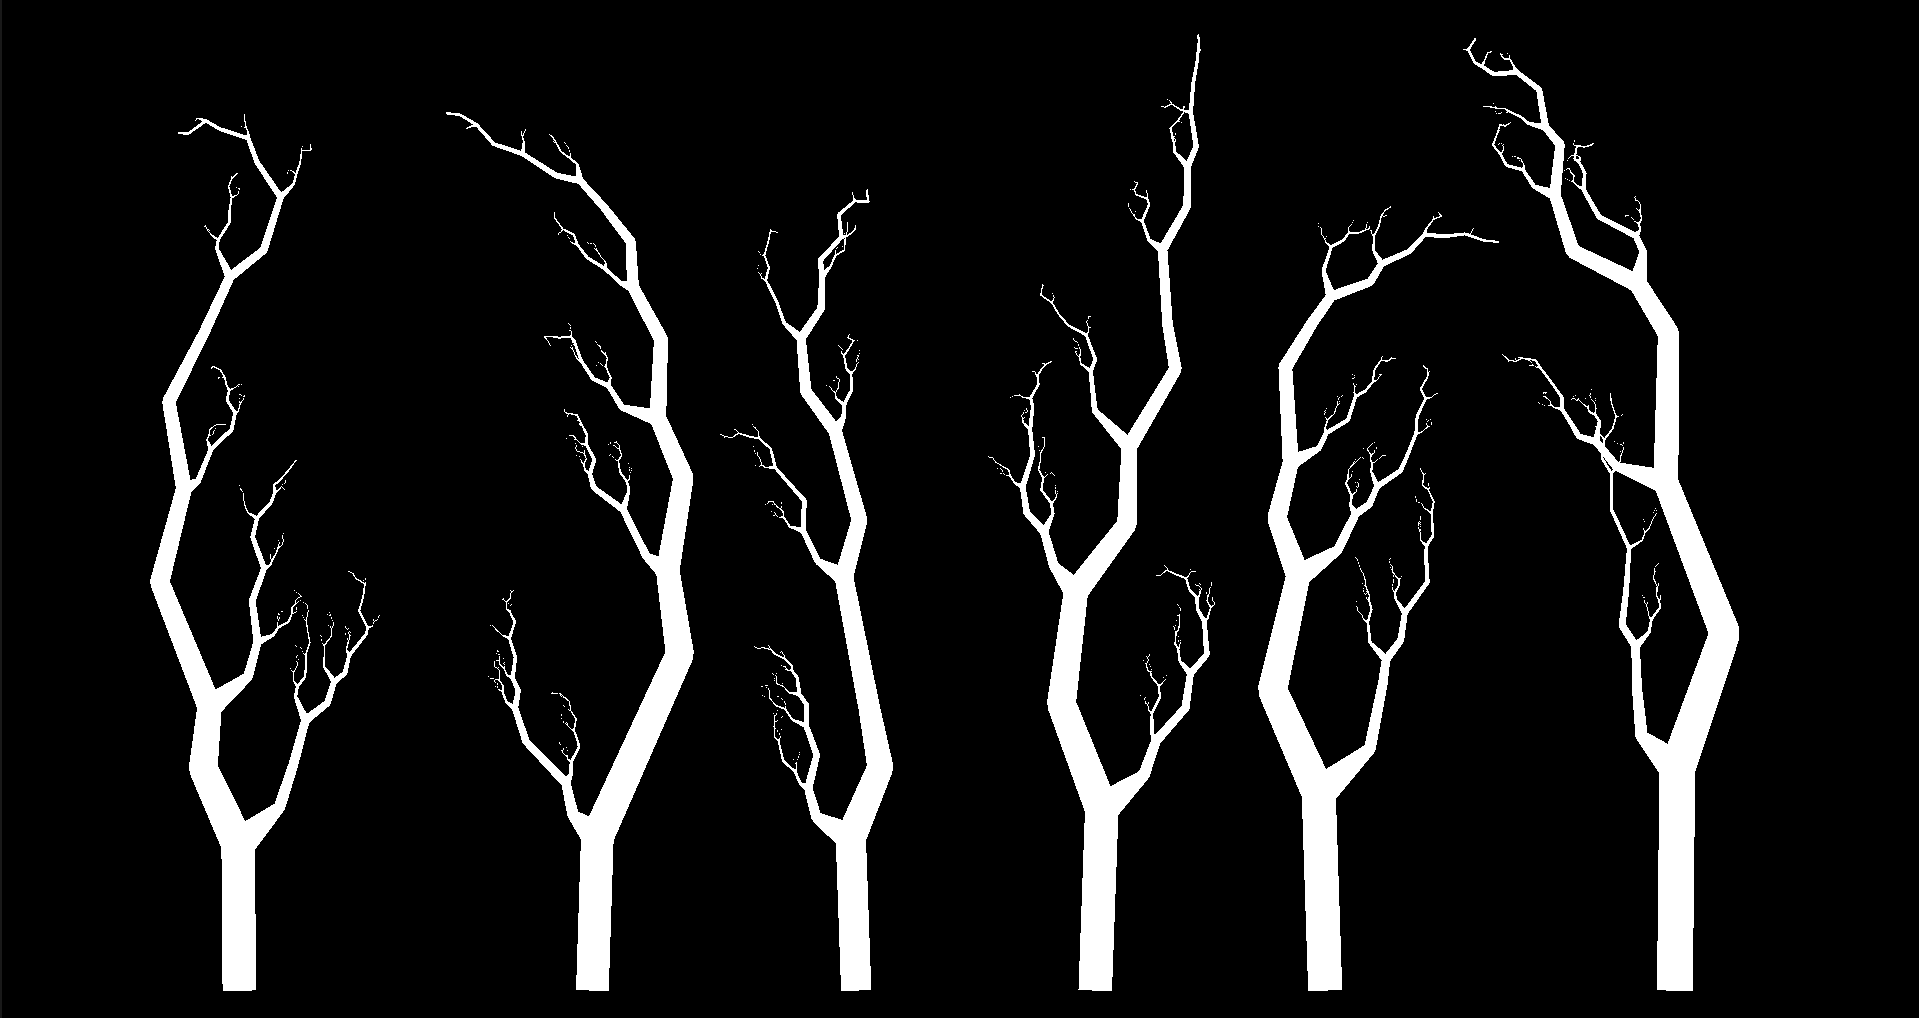
\includegraphics[width=0.66\textwidth]{Blood Vessels}
\caption{\textit{Concrete Earth}'s stochastic model of arterial branching, generated with different seeds.}
\label{Blood Vessels}
\end{figure}

%\begin{figure}[h]
%\centering
%
\includegraphics[width=0.66\textwidth]{Eye Strain Effect}
%\caption{(High-contrast render of) \textit{Concrete Earth}'s eye strain effect.}
%\label{Eye Strain Effect}
%\end{figure}

%\newpage
\subsection{Procedural Narrative} % TECHNIQUE: 'Improv-lite' text generation...

\textit{Concrete Earth} was originally conceived as a work of interactive fiction, a mix of authorship and procedural text generation. Only a fraction of the content has been written so far, so this section will focus on the intended narrative, and the infrastructure \textit{already in place} to facilitate it. 

\subsubsection{Grammars}

Given their origin in linguistics, it is perhaps unsurprising that grammars (see Section \ref{Procedural Screen Shaders}) find use in the field of procedural narrative - \textit{Tracery} \citep{comptonTracery} being a prime example. This is, formally, a stochastic, context-free grammar, with uniformly-distributed production rules for each non-terminal; it iterates a given axiom until all non-terminals (demarcated by \texttt{\{BRACE\}} delimiters) have been replaced. To bemoan the generator as better suited to Twitter bots than interactive storytelling is to misunderstand its design. \citeauthor{comptonTracery} present a lightweight tool that is left \textit{deliberately} narrow, intended for ease-of-use amongst even the most fledgling authors.

\vspace{5pt}\noindent
More substantial works, then, adapt \textit{Tracery}'s grammar-based approach to their own specifications. In \textit{The Annals of the Parrigues}, \citeauthor{shortParrigues} uses a consistent, context-sensitive generator that ``defines any facts about the world that aren’t already defined at the moment of generation'' (\citeyear{shortParrigues}, p. 83). \textit{Voyageur} \citep{diasVoyageur} attaches weightings to the distributions of its production rules \citep{diasVoyageurDescriptions}. Produceral storytelling is an art form; as much as \textit{Concrete Earth} wears the above influences on its sleeve, to try and consolidate these into an `optimal', one-size-fits-all generator would be missing the point. This project therefore uses an implementation of \textit{Tracery} with its own custom modifications.

\paragraph{Recency} To reduce repetition of a word or phrase, one might consider when it has last been used. The custom grammar treats this as a rank: given a non-terminal with $N$ possible production rules, the most recently used rule will have a \textit{recency}\footnote{Or `dryness', as \textit{Improv}, the generator for \textit{Voyageur}, would call it.} of $N-1$, the second most recent $N-2$, and so on down to the rule that was used longest ago (or indeed, never used), with recency $0$. Though it does not account for the intervals between uses, nor the second, third, etc, most recent use, there isn't any reason to overcomplicate a metric that already achieves the desired effect \citep{kazemiSimpleProceduralGeneration}.

\vspace{5pt}\noindent
These ranks are straightforwardly integrating into the production rules' probability distribution. The likelihood of a rule with recency $n$ is scaled by $p^{n/(N-1)}$, such that (all other weightings being equal) the most recently used rule will be $p$ times as likely as the least recent.\footnote{The same string \texttt{alpha} might replace two different non-terminals \texttt{\{A\}}, \texttt{\{B\}}. Recognising these as distinct production rules, the recency with which one was applied to \texttt{\{A\}} has no bearing on when the other is applied to \texttt{\{B\}}, or vice versa.} 

%\vspace{5pt}\noindent
%Note that [joint recency!].

\paragraph{Consistency} Intended to create a feeling of transience, landmarks in \textit{Concrete Earth} can be visited once and once only, and as such do not need tracked by an overall `world model'. The game's approach to characterisation is not so simple. With a narrative largely centred around picking up passengers, journeying with them, then parting ways, it should follow that if a detail about a party member has already been established, the text generator must be able to consistently recover it. %As such,  uses a lightweight approach to consistent characterisation

\vspace{5pt}\noindent
The grammar's \texttt{GenerateSentence} function, therefore, accepts (up to) two pointers to \texttt{StoryCharacter} structs. These are handled by three \textit{consistency markers}: %Not clear enough - relate to braces!
\begin{itemize}[noitemsep]
\item \verb|*|\textit{:} The term \verb|{*A}| tells the grammar to check the first character argument for key \verb|A|. If a value exists, this will be substituted  [If yes; if else], and stored in the character struct for future use.
\item \verb|**|\textit{:} The term \verb|{**A}| similarly applies to the second character argument.
\item \verb|?|\textit{:} %[THIRD EXAMPLE: Consider \verb|{?BARREL #1}-{?BARREL #2}|, (signifying a double-barrelled surname): if 
.\footnote{Note that \texttt{?} can also inherit an empty string, if the preceding non-terminal is not being remembered.}
\end{itemize}



\paragraph{Conditionality} By their very nature, grammars struggle ``to encode high level relationships between different things generated at different points'' in a sentence \citep{cmptn19}. [Explainer of \textit{nested non-terminals}]. [Doesn't scale, but author-friendly enough when it only tracks a few key conditions].

\vspace{5pt}\noindent
Consider how \textit{Concrete Earth}. Using a 
\begin{center}
\begin{BVerbatim}
{*{*GENDER} FORENAME} {*{*GENDER} PATRONYMIC} {*SURNAME}
\end{BVerbatim}
\end{center}
\textit{Concrete Earth}'s grammar processes this as follows:
\begin{enumerate}[label=\textit{\arabic*}\textit{.}, noitemsep]
\item \verb|{*{*GENDER} FORENAME}| $\mapsto$ \verb|{*MASCULINE FORENAME}|\textit{:} The grammar starts with the nested \verb|{*GENDER}| non-terminal. The asterisk tells it to use the character's established gender, but - finding nothing - it randomly decides whether they are a man, woman, or non-binary, and passes this same value into the sentence and the \texttt{StoryCharacter} struct.
\item \verb|{*MASCULINE FORENAME}| $\mapsto$ \verb|LEO|\textit{:} ; even if [never made explicit], the internal consistency
\item \verb|{*{*GENDER} PATRONYMIC}| $\mapsto$ \verb|{*MASCULINE PATRONYMIC}|\textit{:} Now that their gender has been established, the grammar now directly substitutes in the value from the \texttt{StoryCharacter} struct.
\item \verb|{*MASCULINE PATRONYMIC}| $\mapsto$ \verb|NIKOLAYEVICH|\textit{:} The character's forename is matched to a patronymic of the same gender (``Nikolayevich'' here meaning ``Son of Nikolay'') \footnote{As far as this report can tell, there are no gender-neutral patronymics in Russian - without actually speaking the language, it seems most appropriate to drop these from non-binary characters' names entirely. \citet{cook19} offers an invaluable discussion of representation within procedural narrative, and how generators can (whether by accident or authorial intent) reveal prejudices within the societies they create.}
\item \verb|{*SURNAME}| $\mapsto$ \verb|TOLSTOY|\textit{:} The final non-terminal comes with no conditions, and ; this, too, is saved within the
\end{enumerate}
In this case, the grammar terminates after a single iteration. Should \verb|{*BARREL #1}-{*BARREL #2}| (signifying a double-barrelled surname) have replaced \verb|{*SURNAME}|, however, the new non-terminals would needed handled on a second parse.

\vspace{5pt}\noindent
This might feel too limited, from a dramatic perspective. Personality is not immutable; for all this focus on consistency, good storytelling is just as reliant on character \textit{development}. Indeed, as a piece of interactive fiction, the player requires a means of meaningful interaction. The grammar surely requires some sort of override...
%Does this make sense, dramaturgically?

\subsubsection{Content Selection Architectures} 

\textit{Storylets} \citep{kreminskiStorylets} are [definition].

\vspace{5pt}\noindent
In \textit{Concrete Earth}, these storylets are envisioned as the means for these [global changes]. [Discuss a beginning-middle-end structure].%[Though conceptually no different, ... , our `narrative stack'...]
 
\vspace{5pt}\noindent
The current implementation is limited. [Conditions: randomness]. [Effects: entering/exiting the party].

\newpage
\section{Code Organisation}

This application is, amongst over things, a continuation of previous work. Being built on my framework for CMP502, \textit{Concrete Earth} has been a chance to re-evaluate much of my prior code. Shaders, for instance, were once handled with an unwieldy number of C++ classes: a \texttt{LightShader} that passed lighting details into the pixel shader, a \texttt{SkyboxShader} passing in an environment map, etc. These have now been folded back into their parent \texttt{Shader} class, with \texttt{public} functions to turn on the relevant buffers. Though it might seem very basic, identifying and acting on such bad practices early on has been invaluable to the overall development process.

\vspace{5pt}\noindent
Procedural modelling comes with two key challenges - establishing general, multi-purpose frameworks, then applying these to specific use cases. The code has been organised to reflect this dichotomy. While a single , child classes like \texttt{LBloodVessels} and \texttt{LDragonCurves}; the description of how \texttt{MarchingCubes} should be initialized is generated by and passed in as a separate \texttt{Field} class. After initialisation, \texttt{Game.cpp} renders these much as it would any models, handling them within the DirextX pipeline using the preferred vertex and pixel shaders.

\vspace{5pt}\noindent
[The other major point is the board...]

\vspace{5pt}\noindent
The narrative pipeline is as follows. On every move, the \texttt{Board} checks if it should start a new scene. If so, it passes the player's current location (i.e. whether they are near thorns, or a towering monolith) down to the \texttt{StoryEngine}, which in turn receives a . ...passes back up to the \texttt{Board}, having first replaced any non-terminals via its \texttt{Grammar}. The \texttt{Board} then tells the \texttt{StoryEngine} the player's choice, which returns the corresponding consequence (again having been parsed by \texttt{Grammar}).

\vspace{5pt}\noindent
Text events are rendered to the screen with using the ImGui library - the UI is minimal, handled almost entirely within a single \texttt{Game::SetupGUI} function. This application also relies on nlohmann's JSON API.\footnote{Indeed, it is a conscious organisational choice to store word banks of terminals and non-terminals within their own self-contained JSON files, rather than hardcode them into the \texttt{Grammar} itself.} The \href{https://www.dafont.com/benegraphic.font}{\ul{font}} and \href{https://freesound.org/people/JustLaz/sounds/616516/}{\ul{Geiger counter SFX}} were sourced online; the code has been cited as appropriate.

\vspace{5pt}\noindent
Finally, \textit{Concrete Earth} was written with good coding practices in mind. Functions and variables follow a consistent naming convention, focused on readability. The DRY principle has been followed, at least within reason. Even the current, informal use of comments proves effective, these breaking down the logic behind key snippets, highlighting potential bugs, and overall acting as incisive memos-to-self\footnote{This is notably untrue of \texttt{Game.cpp}. All figures in this report have been expressly produced for CMP505 - though unused in the final application, the code used to render these figures remains, commented out in large and unclear blocks solely for the sake of posterity.} (a collaborative project would obviously require a higher standard of documentation). GitHub was used for version control.

%Taking a step back, [...]. [\texttt{Game.cpp} manages three core components: gameplay, UI, and rendering]
%\paragraph{Gameplay} \texttt{Board} [...explain the loop].
%\vspace{5pt}\noindent
%[\texttt{StoryEngine}].
%\vspace{5pt}\noindent
%[Corpora are stored in \texttt{.JSON} files. Accessed by \texttt{nlohmann::json} API].
%\paragraph{UI} [All implemented with ImGui. Simple, stored in \texttt{Game.cpp} itself. This feels appropriate... because of inputs?]
%\paragraph{Rendering}
%\vspace{5pt}\noindent
%Indeed, Section \ref{Features} has been structured [to reflect the two fundamental stages of graphics programming: first implementing frameworks (marching cubes, L-systems), then building tangible objects out of them (terrain hexes, blood vessels)]. \textit{Concrete Earth}'s code is structured accordingly. [Using inheritance...]. [Crucially, little is left exposed in the main \textit{Game.cpp} file...].
%\vspace{5pt}\noindent
%[Furthermore - shaders!]
%\vspace{5pt}\noindent
%[Conclude with existing 5.2 paragraph? Cleaner, more self-contained!]
%\footnote{The notable exception is \texttt{Game.cpp} itself. All figures in this report have been expressly produced for CMP505 - though unused in the final application, code used to render these figures remains, commented out in large blocks for the sake of posterity.}
%Mention use of `tags' in JSON?
%\subsection{Rendering}
%\subsection{GUI}
%[Include HDRR/bloom here...]

\newpage
\section{Evaluation}\label{Evaluation}

\subsection{Features}

If one element of this project constitutes an unambiguous success, it is the L-systems. \textit{Concrete Earth} provides not only a robust framework, but a genuinely interesting use case. Indeed, [...]. Not that there isn't more to do - the procedural animation of the blood vessels, for instance, still feels quite limited - but the \texttt{LSystem} class is in a good place. Above all else, it feels \textit{versatile}, a foundational piece of code that could be carried over to any number of future projects.

\vspace{5pt}\noindent
The role of marching cubes, by contrast, seems much more narrow: height maps have a well-known limitation, to which this algorithm is the well-known solution (see Section \ref{Procedural Terrain}). Implementing the code was a significant technical challenge, but largely successful, and though the generation process does not run especially quickly\footnote{Not on a low-end laptop, at least!} a potential solution has already been identified. \citeauthor{bourkeMarchingTetrahedrons}'s discussion of marching cubes is accompanied by an introduction to \textit{marching tetrahedrons} \citeyearpar{bourkeMarchingTetrahedrons}, a variation of the algorithm that would hopefully improve the efficiency of the code.\footnote{Where there are $256$ possible partitions of a cube, tetrahedrons only come with $2^4 = 16$...} Working within a tetrahedral grid will come with additional nuances (e.g. cell orientation), but I now feel I've built enough intuition to take on this more advanced technique. %To the extent that the feature's performance. Even for moderate values of $n$, \footnote{The complexity of}%one met to great success. To the extent that the performance of the feature can be criticised,  %Marching cubes, too, have been used effectively. T

\vspace{5pt}\noindent
The more interesting question here is how effectively the marching cubes enhance \textit{Concrete Earth}'s setting. As much as they are used to procedurally generate terrain, that terrain can feel somewhat lacking - while this report has already acknowledged the relatively few landmarks available, it's no less notable that they are left untextured. With more time, I would have been keen to write a pixel shader to handle this, but having already experimented with procedural texturing in CMP502 it felt more fruitful to focus on new techniques. Note also that all terrain hexes are generated at runtime; updating these dynamically would be a relatively minor change that greatly reduces repetitivity.

\vspace{5pt}\noindent
\begin{figure}[h]
\centering

\includegraphics[width=0.66\textwidth]{Euclidean Voronoi Voxel}
\caption{3D Voronoi noise. Experiments with voxel textures did not make it past initial prototyping.}
\label{Euclidean Voronoi Voxel}
\end{figure}

\vspace{5pt}\noindent
To the extent that \textit{Concrete Earth} has any single `special feature', though, it would surely be its approach to procedural storytelling. While there's a lot , this has not exactly . For all my interest in \textit{coding} narrative frameworks, I am not myself a writer - a fact reflected in the lack of content available to the grammar. [MORE CONTENT = MORE TESTING]. [Genuinely pleased with the functionality of the grammar]; it is a shame that functionality has not been fully utilised. % While there is a perfectly functional loop of picking up and parting way with new passengers, it is not exactly narrative interesting. 

\vspace{5pt}\noindent
That said, I am genuinely pleased with how the \texttt{Grammar} functions - not so much the surrounding \texttt{Architecture}. 
The same cannot be said of the surrounding \texttt{Architecture}. [The priority was getting a serviceable game loop in place].

\subsection{Code Organisation}

This relates, in part, to a broader organisational problem. [An architecture that grows \textit{with} the content, as my alternative strategy.]

\vspace{5pt}\noindent
[That's not to detract from... - bridge!]. [While the end result of the architecture feels unstructured, overly reliant on special cases... - the rest of the code is good!]

\vspace{5pt}\noindent
More than anything else, I've genuinely tried to . [...]. For instance, [...performance!].

\section{Conclusions}

\vspace{5pt}\noindent
[General lessons]

\vspace{5pt}\noindent
[Features vs. content throughline]

\vspace{5pt}\noindent
[Last: iteration on CMP502...]

\bibliographystyle{agsm}
\bibliography{../../Bibliography/Bibliography}
\addcontentsline{toc}{section}{References}
\end{flushleft}
\end{document}
